\section{Considerações Iniciais}

Como apresentado no Capítulo~\ref{chapter:fundamentacao_teorica}, Seção~\ref{sec:refatoracao}, refatorações são técnicas bem conhecidas que auxiliam desenvolvedores durante a reformulação de um determinado sistema com o objetivo de melhorar atributos internos e ainda possuem a preocupação de preservar o comportamento original do sistema. Em uma linha de pesquisa paralela, como destacado na Seção~\ref{sec:modernizacaoOrientada_Arquitetura} do Capítulo~\ref{chapter:fundamentacao_teorica}, existe a ADM que consiste em nova geração de processos para auxiliar e padronizar as atividades da engenharia reversa; utilizando apenas modelos ao invés de código-fonte como os principais artefatos durante o processo de modernização. O OMG forneça conceitos gerais para a condução de modernização dirigida a modelos por meio da ADM, porém, o grupo OMG não fornece instruções sobre como criar ou aplicar refatorações em instâncias de seus metamodelos. Embora a ADM tenha solicitado um \textit{call for proposal} denominado ADM \textit{Refactoring}\footnote{Até o momento da escrita desta Tese a padronização denominada ADM \textit{Refactoring} estava em estágio de discussão. Assim, uma das principais contribuições deste capítulo é auxiliar na criação e adaptação de soluções de refatorações para o metamodelo KDM.} para propor e desenvolver soluções que auxiliam o engenheiro de modernização durante as atividades de refatorações de sistemas com a utilização do metamodelo KDM até o momento existe uma carência de soluções padronizadas e apoios ferramentais. A ausência de instruções de como criar refatorações já existentes para o metamodelo KDM faz com que engenheiros de modernização criem suas próprias soluções. Usualmente tais soluções tendem a se tornarem proprietárias o que pode dificultar o reúso, diminuindo assim a interoperabilidade, um dos principais objetivos da ADM.

O conjunto de refatoração mais conhecido é o catálogo proposto por~\citeonline{Fowler1999}. Esse catálogo foi proposto primeiramente para ser utilizado em código-fonte, não em modelos, como a UML e KDM. Embora~\citeonline{Fowler1999} tenha criado um catálogo de refatorações para ser utilizado em código-fonte, mais de 60\% das refatorações (44 de 72) são ilustradas e explicadas utilizando modelos. Esta observação levanta a questão se refatorações \aspas{tradicionais}, ou seja, aquelas aplicadas em código-fonte, podem ser criadas para modelos como o KDM. ~\citeonline{Zhang_2005, Boger_2003} afirmam que algumas refatorações, por exemplo, \texttt{Extract Method}, são mais naturais quando executadas diretamente no código-fonte. Outras refatorações, como, \texttt{Rename Class}, \texttt{Pull Up Method}, \texttt{Push Down Method}, etc, podem ser aplicadas tanto em código-fonte quando em modelos; já as refatorações que lidam com herança, tais como \texttt{Extract Class}, \texttt{Extract Interface}, \texttt{Replace Inheritance with Delegation}, são mais intuitivas quando aplicadas diretamente em nível de modelo. 

Embora a refatoração no contexto de modelo tenha alcançado bastante reconhecimento e aceitação na literatura~\cite{Moghadam_2012, Maneerat_2011, Fourati_2011, Einarsson_2012, Steimann_2015, Akiyama_2011, Jensen_2010, Arendt_2012, Millan_2009, Tom_2008_2008}, ainda se faz necessário pesquisas nessa área~\cite{durelli_systematic_mapping, revisao_sistematica_uml_refactoring}. Como já salientado até esse momento existe uma ausência de refatoração e apoios computacionais que auxiliem os engenheiros de modernização e os engenheiros de software a criar, reusar e aplicar refatorações de forma consistente para instâncias do metamodelo KDM. Dessa forma, os engenheiros precisam desenvolver suas próprias refatorações, catálogos e apoios computacionais para refatorar sistemas representados em KDM. Como consequência, essas soluções tornam-se difíceis de serem reutilizadas diminuindo assim a interoperabilidade entre as ferramentas de modernização. 

Diante desse contexto, neste capítulo é apresentado uma abordagem para auxiliar o engenheiro de modernização a criar refatorações para o KDM. Essa abordagem contém um conjunto de diretrizes para auxiliar a criação de refatorações para serem aplicadas em instâncias do metamodelo KDM. Para ilustrar a utilização das diretrizes apresentadas nesse capítulo algumas refatorações proposta por~\citeonline{Fowler1999} são criadas para o metamodelo KDM. Utilizando as diretrizes aqui definidas engenheiros de modernização podem criar refatorações para o metamodelo KDM e facilitar a condução da modernização de um sistema representado como uma instância do metamodelo KDM~\cite{durelli_catalogo, durelli_VEM_ferramenta}. Além das diretrizes e refatorações criadas nesse capítulo também é apresentado uma mapeamento entre o paradigma orientada a objetos (POO) e o metamodelo KDM. Por meio desse mapeamento outros engenheiros de modernização podem adaptar novas refatorações para o metamodelo KDM facilmente. Nota-se que esse capítulo é uma extensão do seguinte artigo: \textit{Towards a Refactoring Catalogue for Knowledge Discovery Metamodel}~\cite{durelli_catalogo}.



%As refatorações apresentadas e adaptadas neste capítulo são baseadas no catálogo de refatoração do~\citeonline{Fowler1999}. O intuito dessas refatorações é facilitar a condução da modernização de um determinado sistema legado representado como uma instância do metamodelo KDM~\cite{durelli_catalogo, durelli_VEM_ferramenta}. Ainda neste capítulo é apresentado um mapeamento entre os conceitos do paradigma orientado a objetos para o metamodelo KDM, assim, engenheiros de modernização podem de forma mais fácil adaptar novas refatorações para o metamodelo KDM. Nota-se que esse capítulo é uma extensão do seguinte artigo: \textit{Towards a Refactoring Catalogue for Knowledge Discovery Metamodel}~\cite{durelli_catalogo}.

%Com o intuito de apresentar e facilitar o entendimento da criação de refatorações para o KDM de uma maneira mais prática, neste capítulo um conjunto de diretrizes são apresentadas. É importante destacar que 

As refatorações aqui criadas são implementadas com o uso da ATL~\cite{Allilaire_06, Jouault_2005, Jouault_2008} e suas restrições (pre- e pós-condições) são implementadas utilizando OCL. ATL e OCL foram escolhidas nesta Tese pois ambas são linguagens bem conhecidas e amplamente utilizadas na literatura. Porém, ressalta-se que as refatorações, bem como as pré- e pós-condições podem ser adaptadas com o uso de outras tecnologias, como, por exemplo, \textit{Query/View/Transformation}~\cite{QVT:OMG}, EMF Henshin~\cite{EMF_Henshin}, SmartQVT~\cite{SmartQVT}, ModelMorf~\cite{ModelMorf}, Kermeta~\cite{kermeta}, \textit{Epsilon Transformation Language}~\cite{ETL_eclipse}, OpenArchitectureWare~\cite{OpenArchitectureWare}, VIATRA~\cite{viatra}, AndroMDA~\cite{andromda} e Fujaba \textit{transformations}~\cite{fujaba}.

As demais seções desta capítulo estão organizadas da seguinte forma: Na Seção~\ref{sec:estrategiasParaAdaptarRefatoracoesParaOMetamodeloKDM} é apresentada as diretrizes aqui propostas para auxiliar os engenheiros de modernização a criar refatorações para o metamodelo KDM. Mais especificadamente, na Subseção~\ref{sec:mapeamento_POO_e_KDM} é apresentado um mapeamento entre os conceitos do POO e as metaclasses do metamodelo KDM; Em seguida as refatorações escolhidas e criadas para o metamodelo KDM são discutidas na Subseção~\ref{sec:refatoracao_para_o_metamodelo_kdm}; Subseção~\ref{sec:linguagemDeTransformacaoUtilizada} é apresenta a linguagem de transformação de modelo que é utilizada para realizar os mecanismos das refatorações; Na Subseção~\ref{sec:linguagem_de_restricao} é apresentado a linguagem de restrição utilizada nas refatorações; Na Subseção\ref{sec:template_refatoracao} é apresentado um \textit{template} para definir refatorações para o metamodelo KDM. Seção~\ref{sec:catalogo_refatoracao_kdm} é apresentado um catálogo de refatoração seguindo as diretrizes destacadas na Seção~\ref{sec:estrategiasParaAdaptarRefatoracoesParaOMetamodeloKDM}. Na Seção~\ref{sec:consideracoes_finais_capitulo_reforacao} as considerações finais desse capítulo são apresentadas.

%\change{terminar aqui. Deve colocar todas as seções bem escritas.}

\section{Diretrizes para Criar Refatorações para Instâncias do Metamodelo KDM}\label{sec:estrategiasParaAdaptarRefatoracoesParaOMetamodeloKDM}

Refatorações aplicadas em nível de modelos são transformações especiais que são aplicadas em instâncias de modelos para melhorar sua estrutura e ainda preservar suas características internas. Esse tipo de refatoração é uma área relativamente nova quando comparada com refatorações aplicadas em código-fonte. Com base em informações obtidas das refatorações tradicionais e de abordagens dirigidas por modelos, foi possível definir diretrizes para auxiliar o engenheiro de modernização a criar refatorações para o metamodelo KDM. As diretrizes apresentadas nesse capítulo utilizam um conjunto de elementos distintos, os quais são essenciais para a criação e definição de refatorações para o contexto da ADM e KDM. Esses elementos são apresentados a seguir:

\begin{itemize}
\item Elementos Estruturais: Mapear os conceitos do POO para o metamodelo KDM (ver Subseção~\ref{sec:mapeamento_POO_e_KDM}). Refatorações são aplicadas em elementos de código, tais como: classes, interfaces, atributos, métodos, etc. Assim, é de suma importância que os engenheiros de modernização saibam identificar quais são as metaclasses em KDM que representam os elementos que serão refatorados;

\item Refatorações: Selecionar um conjunto de refatorações que podem ser adaptadas para o metamodelo KDM (ver Subseção~\ref{sec:refatoracao_para_o_metamodelo_kdm});
Aqui é necessário identificar os elementos do POO que são correspondentes no metamodelo KDM (ver Subseção~\ref{sec:mapeamento_POO_e_KDM});

\item Linguagem de Transformação de Modelo: Utilizar uma linguagem de transformação para a definição e adaptação do mecanismo da refatoração. Refatorações são transformações que são aplicadas em determinadas elementos, no contexto desta Tese em instâncias das metaclasses do KDM. Assim, os elementos estruturais juntamente com a linguagem de transformação de modelo formam o sistema de transformação (ver Subseção~\ref{sec:linguagemDeTransformacaoUtilizada});

\item Linguagem de Restrições: Utilizar uma linguagem de restrição para garantir a preservação de comportamento (semântica e sintaxe) ao aplicar uma refatoração. Instâncias do metamodelo KDM são entidades não executáveis, assim, se faz necessário a utilização de linguagens de restrições para garantir a correta execução da refatoração antes e depois de sua aplicação (ver Subseção~\ref{sec:linguagem_de_restricao});

\item \textit{Template}: Definir um modelo de como as refatorações são informalmente e formalmente apresentadas e documentadas (ver Subseção~\ref{sec:template_refatoracao});

\item Gerenciamento de Consistência: Refatorar uma instância de um determinado modelo pode fazer com que o mesmo fique inconsistente. Para preservar consistência entre as visões da instância do modelo abordagens de preservação de consistência precisam ser adotadas (ver Capítulo~\ref{chapter:Abordagem_de_sincronizacao});

\item Apoio Computacional: Implementar um apoio computacional para auxiliar o engenheiro de software a aplicar a refatoração de forma transparente e instâncias do metamodelo KDM (ver Capítulo~\ref{chapter:ferramenta_kdm_re}).
\end{itemize}

No contexto desta Tese cada refatoração criada para o metamodelo KDM consiste de uma transformação que é executada em uma instância do metamodelo KDM. Além disso, as refatorações também possuem pré- e pós-condições que devem ser satisfeitas antes e depois da transformação/refatoração ser executada. Por exemplo, a refatoração \texttt{Remove ClassUnit} tem como pré-condição que uma determinada instância de \texttt{ClassUnit} deve existir na instância do KDM a ser refatoração e não ser referenciada. Nota-se que a definição de refatoração no contexto desta Tese engloba transformações que preservam o comportamento no contexto de modelos. No contexto do metamodelo KDM a preservação de comportamento é alcançado por meio do pacote \texttt{Action}, o qual é apresentado no Capítulo~\ref{chapter:catalogo_refactoring_KDM}, Seção~\ref{sec:actionPackage}. Além disso, é importante destacar que, apenas a semântica e sintaxe são garantidas e preservadas no contexto de Tese após a aplicação de refatorações no KDM. Garantir que a saída/resultado de um sistema representado por meio do KDM não mude após a aplicação de refatorações não é o objetivo desta Tese uma vez que a instância do KDM não podem ser executada. Neste contexto, apenas as semântica e sintaxe da instância do KDM são preservadas. Dessa forma, a Definição~\ref{def:refatoracao} formaliza refatorações no contexto desta Tese:


\begin{definicao}\label{def:refatoracao}
    \textit{Uma refatoração é uma tripla ordenada $R = (pre, T, pos)$ onde \textbf{pre} é uma asserção (ou seja, pré-condição) que deve ser verdade em uma determinada instância \textbf{R} do metamodelo KDM, \textbf{T} consiste na transformação do modelo \textbf{R}, e \textbf{pos} é a pós-condição a ser aplicada após \textbf{T} ser executada.}
\end{definicao}


Na Figura~\ref{fig:diretrizes_kdm_refatoracao_capitulo} é apresentada uma macro-visão dos elementos utilizados para a criação de refatorações para o KDM utilizando a notação \sigla{SADT}{\textit{Structured Analysis and Design Technique}}~\cite{Marca_1987}. Como observado um conjunto de elementos são utilizados como base para a criação de refatorações para o KDM: elementos estruturais, linguagens de transformações, linguagens de restrições e mapeamento POO - KDM. 

\begin{figure}[h]
	\centering
	% Requires \usepackage{graphicx}
	\caption{Macro-visão para a criação de refatorações para o KDM.}
	\label{fig:diretrizes_kdm_refatoracao_capitulo}
	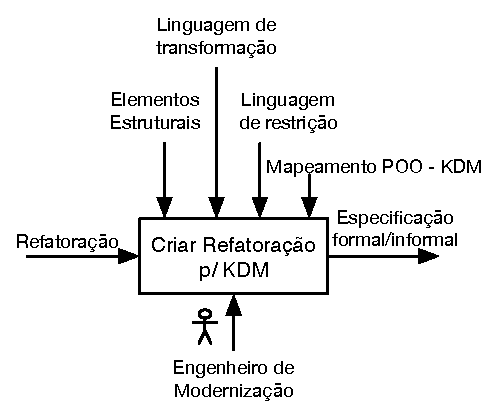
\includegraphics[scale=0.9]{images/novoMacroAbordagemKDMRefactoring}
	\fautor
\end{figure}


Na Figura~\ref{fig:todos_os_passos_diretrizes} uma micro-visão da Figura~\ref{fig:diretrizes_kdm_refatoracao_capitulo} é apresentada. Nota-se que a criação de refatorações para o metamodelo KDM possui cinco principais passos que o engenheiro de modernização deve seguir. Nas subseções a seguir esses passos são apresentadas. %Gerenciamento de consistência e Apoio computacional são apresentados no Capítulo~\ref{chapter:Abordagem_de_sincronizacao} e Capítulo~\ref{chapter:ferramenta_kdm_re}, respectivamente.


\begin{figure}[h]
	\centering
	% Requires \usepackage{graphicx}
	\caption{Diretrizes para criar refatorações para o KDM.}
	\label{fig:todos_os_passos_diretrizes}
	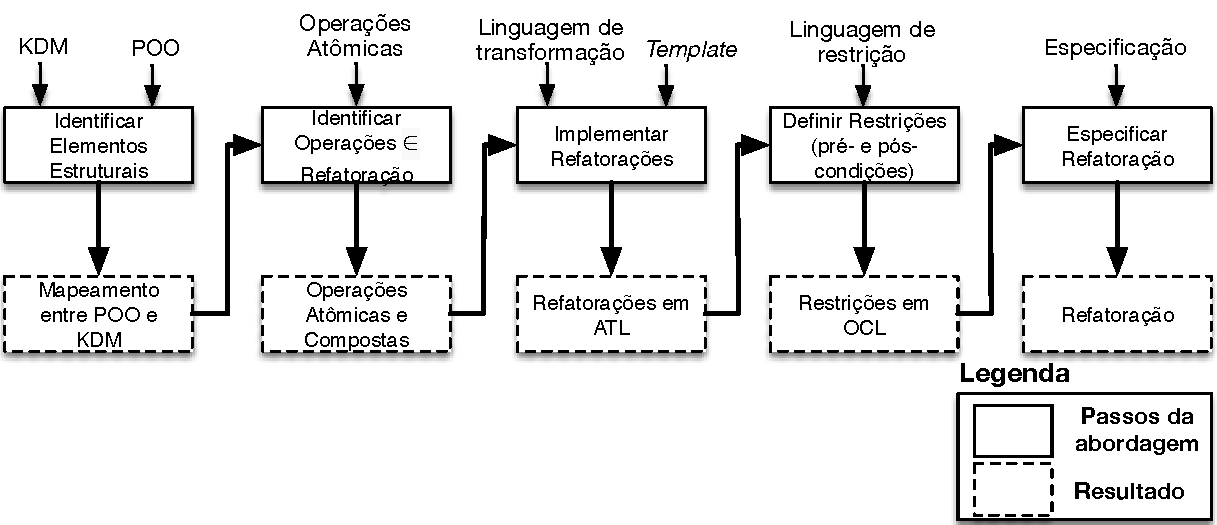
\includegraphics[scale=0.7]{images/novaImagemAbordagemCriarRefatoracao}
	\fautor
\end{figure}

\subsection{Identificar Elementos Estruturais}\label{sec:mapeamento_POO_e_KDM}

Nesta atividade o objetivo é traduzir os conceitos do POO para o metamodelo KDM. É identificado os elementos estruturais do POO em relação as metaclasses disponíveis no metamodelo KDM. De acordo com~\citeonline{Zhang_2005, Boger_2003} um dos maiores desafios quando necessita-se adaptar refatorações para um determinado metamodelo é saber quais são as metaclasses corretas que representam determinadas construções/declarações de um determinado paradigma de programação. É importante identificar se a metaclasse escolhida para fazer a refatoração representa realmente o elemento e o conceito do POO. Dessa forma, antes de realizar a adaptação de qualquer refatoração para o metamodelo KDM, deve-se primeiramente identificar as metaclasses do KDM que têm características similares aos conceitos do POO, bem como instruções comumente utilizadas em todas as linguagens de programação, tais como, ramificações, iterações, etc. 

Um mapeamento entre os conceitos/elementos do POO e as metaclasses do metamodelo KDM foi realizado. Esse mapeamento pode ser visto na Tabela~\ref{tab:mapemanetoEntreOOPeKDM}. Nessa tabela é possível visualizar as metaclasses do metamodelo KDM que possuem características similares aos conceitos/elementos do POO. Utilizando essa Tabela~\ref{tab:mapemanetoEntreOOPeKDM}, engenheiros de modernização podem identificar os elementos estruturais necessários para adaptar as refatorações para o metamodelo KDM. Assim, qualquer exemplo de refatoração definida para o POO pode ser adaptada para o metamodelo KDM. Como observado, a Tabela~\ref{tab:mapemanetoEntreOOPeKDM} contém três colunas: \aspas{Elemento do Código-fonte}, \aspas{Pacote::metaclasse do KDM} e \aspas{Descrição}. A primeira coluna informa a construção da linguagem de programação (\textit{statement})e/ou o conceito do POO (pacote, classe, interface, etc), respectivamente. Em seguida a coluna \aspas{Pacote::metaclasse do KDM} apresenta a metaclasse responsável por mapear a construção e/ou o conceito do POO. Note que essa coluna segue o formato \aspas{\textit{Package}::\textit{Meta-class}}. A ultima coluna, \aspas{Descrição}, possui informações sobre a metaclasse, tais como: seu propósito, seus meta-atributos e suas meta-associações.

\begin{longtable}[c]{| m{1.9cm} | m{3.57cm}| m{9.3cm} |}
 \caption{Mapeamento entre POO e metaclasses do metamodelo KDM.\label{tab:mapemanetoEntreOOPeKDM}}\\
 
 \hline
 \multicolumn{3}{| c |}{Início da Tabela}\\
 \hline
 Elemento do Código-Fonte & Pacote::metaclasse do KDM & Descrição\\
 \hline
 \endfirsthead
 
 \hline
 \multicolumn{3}{|c|}{Continuação da Tabela~\ref{tab:mapemanetoEntreOOPeKDM}}\\
 \hline
 Elemento do Código-Fonte & Pacote::metaclasse do KDM & Descrição\\
 \hline
 \endhead
 
 \hline
 \endfoot
 
 \hline
 \multicolumn{3}{| c |}{Fim da Tabela~\ref{tab:mapemanetoEntreOOPeKDM}}\\
 \hline\hline
 \endlastfoot
 
 Pacote & code::Package & A metaclasse \texttt{Package} é um contêiner para elementos de programa, como classes e interfaces. Essa metaclasse contém um principal meta-atributo, \texttt{name}, que especifica o nome do pacote. Além disso, esta metaclasse possui uma principal meta-associação \texttt{codeElement:AbstractCodeElement[0..*]} onde, pacotes, classes e interfaces podem ser incluídos. \\ 
\hline
Classe & code::ClassUnit & A metaclasse \texttt{ClassUnit} possui dois principais meta-atributos,  \texttt{name:String} e \texttt{isAbstract:boolean}. O primeiro é utilizado para especificar o nome da classe, o segundo é utilizado para informar se a classe é ou não abstrata. Além disso, essa metaclasse possui três meta-associações: \texttt{attribute:Attribute[0..*]}, \texttt{codeRelation:KDMRelationship[0..*]} e  \texttt{codeElement:AbstractCodeElement[0..*]}. \texttt{attribute} é utilizado para especificar a  visibilidade da classe, ou seja, \textit{public}, \textit{private}, ou \textit{protected}. \texttt{codeRelation} agrupa todos os relacionamentos que uma determinada classe possui, por exemplo, heranças e associações. \texttt{codeElement} agrupa qualquer metaclasse cujo tipo é uma concretização de \texttt{AbstractCodeElement}, como: \texttt{StorableUnit}, \texttt{MethodUnit}, \texttt{MemberUnit}, etc. \\ 
\hline
Interface & code::InterfaceUnit & A metaclasse \texttt{InterfaceUnit} possui características similares a metaclasse \texttt{ClassUnit}, porém, não tem o meta-atributo \texttt{isAbstract}, uma vez que todas as interfaces são abstratas por padrão. \\ 
\hline
Atributo & code::StorableUnit & A metaclasse \texttt{StorableUnit} possui dois principais meta-atributos: \texttt{name:String} e \texttt{kind:StorableKind}. Similarmente, esse metaclasse possui duas principais meta-relacionamentos: \texttt{attribute:Attribute[..*]} e \texttt{type:DataType[1]}. \texttt{name} é utilizado para especificar o nome do atributo. \texttt{kind} é uma enumeração utilizada para especificar propriedades do atributo, ou seja, informar se o mesmo é local, global, estático, etc. \texttt{attribute} é utilizado para definir o escopo do atributo, \textit{public}, \textit{private}, ou \textit{protected}. E \texttt{type} é utilizado para definir o tipo do atributo.  \\ 
\hline
Método & code::MethodUnit & A metaclasse \texttt{MethodUnit} possui dois principais meta-atributos: \texttt{name:String} e \texttt{kind:MethodKind}. \texttt{name} é utilizado para especificar o nome do método. \texttt{kind} é uma enumeração utilizada para especificar propriedades do método, ou seja, informar se o método é \textit{construtor}, \textit{destructor}, \textit{virtual}, \textit{abstract}, etc. Similarmente, esse metaclasse possui dois principais meta-relacionamentos: \texttt{attribute:Attribute[..*]}, \texttt{codeElement:AbstractCodeElement[0..*]}. \texttt{attribute} é utilizado para definir o escopo do método - informar se o mesmo é \textit{public}, \textit{private}, ou \textit{protected}. E \texttt{codeElement} é utilizado para agrupar declarações internas do método, ou seja, assinatura do método, bloco do método, etc.\\ 
\hline
Assinatura do Método & code::Signature & A metaclasse \texttt{Signature} possui um principal meta-atributo, \texttt{name:String}, o qual é utilizado para especificar o nome do método. Além disso, essa metaclasse contém um principal meta-relacionamento denominado \texttt{parameterUnit:ParameterUnit[..*]} que é utilizado para especificar os parâmetros que o método possui.\\ 
\hline
Bloco do Método & action::BlockUnit & A metaclasse \texttt{BlockUnit} representa blocos lógicos e físicos relacionados, por exemplo, blocos de instruções \textit{if}, \textit{for}, \textit{while}, etc. Possui um meta-relacionamento denominado \texttt{codeElement:AbstractCodeElement[0..*]} que é utilizado para agrupar qualquer instruções lógicas ou físicas.\\ 
\hline
Parâmetro & code::ParameterUnit & A metaclasse \texttt{ParameterUnit} pode representar o nome, tipo e a posição dos parâmetros em uma assinatura de método. além de permitir o tipo de parâmetro (valor ou referência). Essa metaclasse contém dois principais meta-atributos: \texttt{name:String} e \texttt{kind:ParameterKind}. O primeiro meta-atributo representa o nome do parâmetro, o segundo meta-atributo é uma enumeração para especificar o tipo de parâmetro (valor ou referência). Além disso, \texttt{ParameterUnit} possui o meta-relacionamento \texttt{type:DataType[1]} para especificar o tipo do parâmetro, esse tipo pode ser tipos primitivos ou outros tipos.\\ 
\hline
Associação & code::HasType & A metaclasse \texttt{HasType} representa relação semântica entre um elemento de dados e seu tipo. Essa meta-calsse possui duas principais meta-relacionamentos: \texttt{from:CodeItem} e \texttt{to:DataType}.\\ 
\hline
Herança \texttt{extends} & code::Extends & A metaclasse \texttt{Extends} representa relação semântica de herança entre duas \texttt{ClassUnits} ou duas \texttt{InterfaceUnits}. Essa relação semântica é representada por dois meta-relacionamentos: \texttt{from:DataType} e \texttt{to:DataType}.\\ 
\hline
Herança \texttt{implements} & code::Implements & A metaclasse \texttt{Implements} representa relação semântica de herança entre uma \texttt{ClassUnit} e uma \texttt{InterfaceUnit}. Similarmente a metaclasse \texttt{Extends} a relação semântica é representada por dois meta-relacionamentos: \texttt{from:DataType} e \texttt{to:DataType}.\\ 
\hline
\textit{if}, \textit{for}, \textit{while}, etc & action::ActionElement & \texttt{ActionElement} representa instruções e declarações de uma determinada linguagem de programação, ou seja, pode ser utilizada para representar ramificações, iterações, etc. \texttt{ActionElement} possui um principal meta-atributo denominado \texttt{kind:String} que representa qual o tipo instrução que a metaclasse esta representando. Essa metaclasse possui dois meta-relacionamentos \texttt{codeElement:AbstractCodeElement[0..*]} e \texttt{actionRelation:ActionRelationship[0..*]}.\\ 
\hline
 \end{longtable}


Na Tabela~\ref{tab:mapemanetoEntreOOPeKDM} é possível ver a relação existente entre os conceitos do POO, bem como algumas instruções de linguagens de programação e as algumas metaclasses do metamodelo KDM. Para atender aos objetivos deste trabalho a Tabela~\ref{tab:mapemanetoEntreOOPeKDM} apresenta apenas as principais metaclasses do KDM que são utilizadas nas refatorações aqui adaptado, uma vez que seria inviável mapear todas as noventa metaclasses do metamodelo KDM.

Como apresentado na Tabela~\ref{tab:mapemanetoEntreOOPeKDM} algumas metaclasses podem ser diretamente mapeadas com elementos do POO, tais como: classes (\texttt{ClassUnit}), interfaces (\texttt{InterfaceUnit}), atributos (\texttt{StorableUnit}), métodos (\texttt{MethodUnit}), etc. Entretanto, como o KDM tem como objetivo ser um metamodelo independente de plataforma para representar de forma genérica todas as abstrações e paradigmas de programação, algumas construções de programação não possuem uma metaclasse particular. Por exemplo, iterações e ramificações em KDM são representadas utilizando a mesma metaclasse, \texttt{ActionElement}. Esse mapeamento ocorre pois o KDM define uma metaclasse genérica para especificar ramificações e iterações para preservar a independência de plataforma; seria inviável para o metamodelo definir específicas metaclasses para representar ramificações e iterações uma vez que cada linguagem de programação possui um determinada particularidade. Para que o mapeamento fique o mais genérico e independente de plataforma possível a metaclasse \texttt{ActionElement} utiliza o meta-atributo \texttt{kind} que possui os seguintes valores: \textit{variable declaration}, \textit{if}, \textit{for}, \textit{while}, etc.

Com a utilização da Tabela~\ref{tab:mapemanetoEntreOOPeKDM} o engenheiro de modernização pode agora escolher qual refatoração criar para o metamodelo KDM. É de suma importância identificar previamente qual elemento do metamodelo KDM será utilizado durante a refatoração para o engenheiro criar e implementar a refatoração como apresentado na Seção~\ref{sec:linguagemDeTransformacaoUtilizada}. Por exemplo, suponha que o engenheiro de modernização almeja criar a refatoração \texttt{Rename Method}. Dessa forma, utilizando a Tabela~\ref{tab:mapemanetoEntreOOPeKDM} pode-se observar qual é a metaclasse em KDM que representa métodos; métodos em KDM são representados por instâncias da metaclasse \texttt{MethodUnit}, assim, a refatoração torna-se \texttt{Rename MethodUnit}. Adicionalmente, por meio da Tabela~\ref{tab:mapemanetoEntreOOPeKDM} é possível identificar todos os relacionamentos que a metaclasse \texttt{MethodUnit} possui, os quais podem ser úteis durante a implementação da refatoração.


\subsection{Identificar Operações}\label{sec:refatoracao_para_o_metamodelo_kdm}

Após identificar todos os elementos estruturais e identificar o mapeamento entre POO e o metamodelo KDM, o próximo passo é identificar as operações que compõem a refatoração a ser criada. Como já salientado, no contexto desta Tese todas as refatorações são transformações que são realizadas em instâncias do KDM. Assim, as refatorações podem ser agrupadas em nível de sua granularidade. As granularidades podem ser definidas em dois níveis de operações: (\textit{i}) operações atômicas e (\textit{ii}) operações compostas. As granularidades definidas como operações atômicas podem ser especificadas por meio de operações primitivas que são executadas na instância do metamodelo KDM. Tais operações primitivas são listadas a seguir



%escolher qual refatoração criar. Dessa forma, nesta seção algumas refatorações propostas por~\citeonline{Fowler1999} foram escolhidas para serem adaptadas para o contexto do metamodelo KDM. As refatorações propostas por~\citeonline{Fowler1999} foram escolhidas para serem adaptas para o contexto do metamodelo KDM uma vez que são bem conhecidas, básicas e de baixa granularidade. As refatorações adaptadas seguem a mesma convenção de nomenclatura definida por~\citeonline{Fowler1999}. Porém, os nomes de algumas refatorações foram alteradas para indicar o metamodelo KDM como seu novo domínio de aplicação, por exemplo, \texttt{MoveMethod} torna-se \texttt{MoveMethodUnit} e \texttt{MoveAttribute} torna-se \texttt{MoveStorableUnit}, etc. 

%No contexto desta Tese todas as refatorações são transformações que são realizadas em uma instância do metamodelo KDM. Assim, as refatorações podem ser agrupadas em nível de sua granularidade. As granularidades podem ser definidas em dois níveis de operações: (\textit{i}) operações atômicas e (\textit{ii}) operações compostas. As granularidades definidas como operações atômicas podem ser especificadas por meio de operações primitivas que são executadas na instância do metamodelo KDM. Tais operações primitivas são listadas a seguir:

\begin{itemize}
\item \texttt{add}: qualquer operação que adicione uma instância de uma metaclasse do metamodelo KDM (ver Tabela~\ref{tab:mapemanetoEntreOOPeKDM});
\item \texttt{delete}: qualquer operação que remove uma instância de uma metaclasse do metamodelo KDM (ver Tabela~\ref{tab:mapemanetoEntreOOPeKDM});
\item \texttt{change}: qualquer operação que altere um valor de um meta-atributo de uma metaclasse do metamodelo KDM (ver Tabela~\ref{tab:mapemanetoEntreOOPeKDM}).
\end{itemize}

As refatorações de granularidade compostas consistem em uma combinação de operações atômicas. Por exemplo, considere a refatoração \texttt{Move ClassUnit}, essa refatoração compõe-se de duas operações atômicas: \texttt{add} e \texttt{delete}. Por exemplo, uma nova instância da metaclasse \texttt{ClassUnit} deve ser adicionada no local onde se almeja mover essa instância e em seguida deve-se aplicar a operação atômica \texttt{delete} na instância da metaclasse \texttt{ClassUnit} antiga. Similarmente, por meio da junção dessas operações atômicas é possível criar e adaptar refatorações já existentes na literatura para o KDM. Por exemplo, considere as refatorações propostas por~\citeonline{Fowler1999}. Essa refatorações podem ser facilmente adaptas para o contexto do metamodelo KDM uma vez que são bem conhecidas, básicas e de baixa granularidade. Na Tabela~\ref{tab:refatoringsCatalogo} algumas das refatorações propostas por~\citeonline{Fowler1999} são apresentadas ressaltando a granularidade da refatoração e qual(is) a(s) operação(ões) que devem ser utilizadas para criar a refatoração. Note que as refatorações apresentada nessa tabela seguem a mesma convenção de nomenclatura definida por~\citeonline{Fowler1999}. Porém, os nomes de algumas refatorações foram alteradas para indicar o metamodelo KDM como seu novo domínio de aplicação, por exemplo, \texttt{MoveMethod} torna-se \texttt{MoveMethodUnit} e \texttt{MoveAttribute} torna-se \texttt{MoveStorableUnit}, etc.


%Na Tabela~\ref{tab:refatoringsCatalogo} as refatorações que podem ser facilmente criadas para o metamodelo KDM são apresentadas.

\begin{table}[h]
\caption{Refatorações adaptadas para o metamodelo KDM.\label{tab:refatoringsCatalogo}}
\begin{center}
\begin{tabular}{ | m{4.5cm} | m{2.5cm} | m{4cm}| } 
\hline
\multicolumn{1}{|c|}{Refatoração} & \multicolumn{1}{|c|}{Granularidade} & \multicolumn{1}{|c|}{Tipo de Operação}\\ 
\hline
\textit{Add Package} &  Atômica & \texttt{add}\\ 
\hline
\textit{Add ClassUnit} &  Atômica & \texttt{add}\\ 
\hline
\textit{Add StorableUnit} &  Atômica & \texttt{add}\\ 
\hline
\textit{Add MethodUnit} &  Atômica & \texttt{add}\\ 
\hline
\textit{Delete Package} &  Atômica & \texttt{delete}\\ 
\hline
\textit{Delete ClassUnit} &  Atômica & \texttt{delete}\\ 
\hline
\textit{Delete StorableUnit} &  Atômica & \texttt{delete}\\ 
\hline
\textit{Delete MethodUnit} &  Atômica & \texttt{delete}\\ 
\hline
\textit{Rename Package} &  Atômica & \texttt{change}\\ 
\hline
\textit{Rename ClassUnit} &  Atômica & \texttt{change}\\ 
\hline
\textit{Rename StorableUnit} &  Atômica & \texttt{change}\\ 
\hline
\textit{Rename MethodUnit} &  Atômica & \texttt{change}\\ 
\hline
\textit{Move StorableUnit} &  Composta & \texttt{add} $|$ \texttt{delete}\\ 
\hline
\textit{Move MethodUnit} &  Composta & \texttt{add} $|$ \texttt{delete}\\ 
\hline
\textit{Extract ClassUnit} &  Composta & \texttt{add} $|$ \texttt{delete} $|$ \texttt{change}\\
\hline
\textit{Inline ClassUnit} &  Composta & \texttt{change} $|$ \texttt{delete}\\ 
\hline
\textit{Flatten Hierarchy} &  Composta & \texttt{add} $|$ \texttt{delete} $|$ \texttt{change}\\ 
\hline
\textit{Push Down MethodUnit} &  Composta & \texttt{add} $|$ \texttt{delete}\\ 
\hline
\textit{Push Down StorableUnit} &  Composta & \texttt{add} $|$ \texttt{delete}\\ 
\hline
\textit{Pull Up MethodUnit} &  Composta & \texttt{add} $|$ \texttt{delete}\\
\hline
\textit{Pull Up StorableUnit} &  Composta & \texttt{add} $|$ \texttt{delete}\\
\hline
\textit{Extract SubClass} &  Composta & \texttt{add} $|$ \texttt{change}\\
\hline
\textit{Encapsulate StorableUnit} &  Composta & \texttt{add} $|$ \texttt{change}\\
\hline
\end{tabular}
\end{center}
\end{table}

Após o engenheiro de modernização escolher qual refatoração irá criar para o metamodelo KDM e identificar qual(is) é(são) a(s) operação(ões) que compõe(m) a refatoração escolhida o próximo passo é a implementação da refatoração utilizando técnicas e linguagem de transformação em modelo. Na próxima seção maiores informações são apresentadas.

\subsection{Implementar Refatoração}\label{sec:linguagemDeTransformacaoUtilizada}

Na literatura é possível identificar um conjunto de técnicas e linguagens específicas para auxiliar a condução e especificação de transformação de modelos~\cite{Biehl_2010, Mens_2006, Allilaire_06}. As duas abordagens mais utilizadas na literatura para a elaboração e condução de transformações/refatoração de modelos são: (\textit{i}) abordagem de manipulação direta e (\textit{ii}) abordagem de transformação genérica. A primeira abordagem utiliza linguagens de programação tradicional para a aplicação das refatorações. Ferramentas que utilizam essa abordagem utilizam linguagens como Java, C, C++ etc~\cite{Bruneliere_2014}. Usualmente tais linguagens proporcionam uma infraestrutura mínima para organizar as transformações. Algumas características de suma importância para refatorações de modelo como, regras de transformações, preservação de comportamento são, usualmente criadas pelo engenheiro, uma vez que tais linguagens não possuem API para lidar com tais características. Dessa forma, refatorações que utilizam essa abordagem tornam-se dependente de plataformas, afetando assim a reusabilidade das refatorações. 

A segunda abordagem, transformação genérica, utiliza linguagens desenvolvidas especialmente para realizar transformações em modelos, tais como ATL, QVT, Kermeta, etc. Usualmente, tais abordagens são conhecidas como endógenas e são implementadas utilizando técnicas de reescrita de grafo (ver Capítulo~\ref{chapter:fundamentacao_teorica} Seção~\ref{sec:transformacoes_de_modelos}). Diferentemente da primeira abordagem, a segunda abordagem facilita o reúso de refatorações. Por exemplo, utilizando a segunda abordagem o engenheiro de modernização pode criar um conjunto de regras de refatorações por meio de linguagens de transformações genéricas, assim, tais refatorações podem ser invocadas utilizando qualquer linguagem de programação. O engenheiro pode escrever um código em Java que tem como entrada uma instância do metamodelo KDM para ser refatorado, a reforação a ser aplicada nessa instância e um conjunto de parâmetros para realizar a refatoração na instância do metamodelo KDM.

Dado essa motivação, no contexto desta Tese, a segunda abordagem é utilizada. Mais especificamente a linguagem de transformação ATL~\cite{ATL_eclipse,Jouault_2008} foi escolhida para definir e implementar refatorações em instâncias do metamodelo KDM. ATL foi escolhida como linguagem de transformação considerando vários aspectos. Essa linguagem está integrada na plataforma Eclipse, o que fornece uma série de recursos padrões para o desenvolvimento (\textit{syntax highlighting} e \textit{debugger}). ATL é parte do projeto \textit{Model-To-Model} e possui um grupo de discussão ativo, constantemente atualizado, vários exemplos e diversos estudos de casos aplicados até mesmo na indústria utilizam tais linguagens.


ATL possui um modulo de execução denominado \textit{refining} que é utilizado para criar refatorações em nível de modelo. Esse modulo foi introduzido para facilitar a programação de (ou refatoração) transformações. Com o modulo \textit{refining}, os engenheiros de modernização podem se concentrarem no código ATL dedicada à geração de elementos estruturados modificados. Outros elementos estruturados do KDM (por exemplo, aqueles que permanecem inalteradas antes e após a refatoração) são implicitamente processados pelo mecanismo de ATL. O modulo \textit{refining} pode ser utilizado simplesmente substituindo a palavra-chave \texttt{from} pela palavra-chave \texttt{refining}. Obviamente, o modo de \textit{refining} só pode ser utilizado para as transformações endógenas (\aspas{\textit{in-place}}) (ver Capítulo~\ref{chapter:fundamentacao_teorica}, Seção~\ref{sec:transformacoes_de_modelos})


Como apresentado na Seção~\ref{sec:refatoracao_para_o_metamodelo_kdm} as refatorações são agrupadas em dois níveis de operações: (\textit{i}) operações atômicas e (\textit{ii}) operações compostas. As granularidades definidas como operações atômicas são: \texttt{add}, \texttt{delete} e \texttt{change}. Essas operações atômicas podem ser facilmente implementadas em ATL. Dessa forma, um \textit{template} para cada operação atômica é disponibilizado como artefato para auxiliar o engenheiro de modernização a criar genericamente refatorações para o KDM. O \textit{template} para a operação atômica \texttt{add} é apresentado no Código-fonte~\ref{codigo:template_addKDMElement}. As partes fixas dos \textit{templates} são formadas por texto ATL e as partes variantes são formadas por três tipos de instruções: (\textit{i}) argumentos, \textbf{ArgX}\footnote{\textbf{ArgX}, onde \textbf{X} representa um número sequencial do argumentos. \label{foot:Arg}}, demarcadas pelos símbolos \aspas{\textbf{<\#}} e \aspas{\textbf{\#>}} e que devem ser substituídos por \textit{strings} validas na linguagem ATL; (\textit{ii}) argumentos, \textbf{ArgX}\textsuperscript{\ref{foot:Arg}}, demarcadas pelos símbolos \aspas{\textbf{<\%}} e \aspas{\textbf{\%>}} e que devem ser substituídos por metaclasses do metamodelo KDM, por exemplo, \texttt{ClassUnit}, \texttt{InterfaceUnit}, \texttt{StorableUnit}, \texttt{MethodUnit}, etc; e (\textit{ii}) argumentos, \textbf{ArgX}\textsuperscript{\ref{foot:Arg}}, demarcados pelos símbolos \aspas{\textbf{<$@$}} e \aspas{\textbf{@>}} que devem ser substituídos de acordo com o domínio do sistema que será aplicado a refatoração, por exemplo, nomes de pacotes, classes, interfaces, atributos, métodos, etc.  

%argumentos, \textbf{ArgX} onde X representa um número cardinal, demarcadas pelos símbolos \aspas{\textbf{<\%}} e \aspas{\textbf{\%>}} ou \aspas{\textbf{<$@$}} e \aspas{\textbf{@>}}. O primeiro símbolo (\aspas{\textbf{<\%}} e \aspas{\textbf{\%>}}) informa para o engenheiro de modernização que metaclasses do KDM devem ser substituídas pelo argumento.

%Deve-se também utilizar outro artefato para auxiliar o engenheiro de modernização a substituir as partes variáveis do \textit{template} de forma correta.

%Outro artefato que deve ser utilizado juntamente com o \textit{template} apresentado no Código-fonte~\ref{codigo:template_addKDMElement} para auxiliar o engenheiro de modernização a criar a operação atômica é a Tabela X. Essa tabela é utilizada como um guia para conduzir o engenheiro de modernização a especificar corretamente os as partes variantes do \textit{template}, ou seja, os argumentos.


\begin{table}
\centering
\caption{Guia para auxiliar a substituir os argumentos do \textit{template} apresentado no Código-fonte~\ref{codigo:template_addKDMElement}.}
\label{tab:guia_template_operacao_add}
\begin{tabular}{ | m{1.7cm} | m{12cm}| } 
\hline
\multicolumn{1}{|c|}{Argumentos}                                         & \multicolumn{1}{c|}{Valores} \\ \hline
\multicolumn{1}{|c|}{\textbf{<\#Arg1\#>}} & Nome do módulo. Pode-se utilizar qualquer \textit{string} válida na linguagem ATL; \\ 
\hline
\multicolumn{1}{|c|}{\textbf{<\#Arg2\#>}} & Nome da regra. Pode-se utilizar qualquer \textit{string} válida na linguagem ATL; \\  
\hline
\multicolumn{1}{|c|}{\textbf{<\%Arg3\%>}} & Nome de uma metaclasse (\texttt{ClassUnit}, \texttt{InterfaceUnit}, \texttt{StorableUnit}, \texttt{MethodUnit}, etc). Deve-se especificar o nome da metaclasse que conterá a nova instância da metaclasse a ser criada; \\ 
\hline
\multicolumn{1}{|c|}{\textbf{<$@$Arg4@>}} & Nome da instância do elemento estrutural especificado no \textbf{<\%Arg3\%>}. Deve-se especificar o nome da instância da metaclasse que conterá a nova instância da metaclasse a ser criada. Esse argumento depende do domínio do sistema que será aplicado a refatoração e é identifica no meta-atributo \texttt{name} das metaclasses do KDM;  \\ 
\hline
\multicolumn{1}{|c|}{\textbf{<\%Arg5\%>}} & Nome de uma metaclasse que será instanciado. Deve-se especificar o nome da metaclasse que será criada;  \\ 
\hline
\multicolumn{1}{|c|}{\textbf{<$@$Arg6@>}} & Nome da nova instância que será criada. Deve-se especificar o nome da instância da metaclasse que será criada. Esse argumento também depende do domínio do sistema que será aplicado a refatoração.  \\ 
\hline
\end{tabular}
\end{table}


\begin{codigo}[caption={[\textit{Template} ATL para realizar a operação atômica \texttt{add}.] \textit{Template} ATL para realizar a operação atômica \texttt{add}.},escapeinside={(*@}{@*)}, basicstyle=\footnotesize, label={codigo:template_addKDMElement}, language=ATL]{Name}
module (*@<\textbf{\#Arg1\#}>@*);
create OUT : MM refining IN : MM;
rule create(*@<\textbf{\#Arg2\#}>@*){
	from
		source : MM!(*@<\textbf{\%Arg3\%}>@*) (source.name = (*@<\textbf{$@$Arg4@}>@*))
	to 
		target: MM!(*@<\textbf{\%Arg3\%}>@*) (
			codeElement (*@$\leftarrow$@*) source.codeElement(*@$\rightarrow$@*)including(newElement)
		),
		newElement: MM!(*@<\textbf{\%Arg5\%}>@*) (
			name (*@$\leftarrow$@*) (*@<\textbf{$@$Arg6@}>@*)
		)
}
\end{codigo}


%para adicionar uma nova instância da metaclasse \texttt{ClassUnit} denominada \texttt{\aspas{novaClassUnit}} no pacote \texttt{com.br.teste}. Como pode ser observado na linha 5 é especificado o nome do pacote (\texttt{\aspas{com.br.teste}}) que é onde a nova instância da \texttt{ClassUnit} será adicionada. A linha 8 representa que a nova instância da \texttt{ClassUnit} será adicionada no associação \texttt{codeElement}. Nas linhas 10-12 uma nova instância da metaclasse \texttt{ClassUnit} é adicionada e seu nome definido como \aspas{novaClassUnit}.

%Mostrar que o Engenheiro de modernização pode adaptar qualquer elemento... Mostrar uma exemplo em ATL onde pode ser substituido pela metaclasse do KDM........

Além do \textit{template} apresentado no Código-fonte~\ref{codigo:template_addKDMElement} outro artefato também deve ser utilizado para auxiliar o engenheiro de modernização a substituir as partes variáveis do \textit{template} de forma correta. Esse artefato é apresentado na Tabela~\ref{tab:guia_template_operacao_add}. Essa tabela é utilizada como um guia para conduzir o engenheiro de modernização a especificar corretamente as partes variantes do \textit{template}, ou seja, os argumentos.

Dado o \textit{template} apresentado no Código-fonte~\ref{codigo:template_addKDMElement}, bem como as Tabelas~\ref{tab:mapemanetoEntreOOPeKDM} e~\ref{tab:guia_template_operacao_add} a combinação desses três artefatos auxilia/guia o engenheiro de software a criar a operação atômica \texttt{add} para um determinado elemento estrutural do KDM, ou seja, \texttt{ClassUnit}, \texttt{InterfaceUnit}, \texttt{Package}, \texttt{StorableUnit}, \texttt{MethodUnit}, etc. Por exemplo, 
%
%
%quando combinado com a Tabela~\ref{x} (os elementos estruturais \texttt{ClassUnit}, \texttt{InterfaceUnit}, \texttt{Package}, \texttt{StorableUnit}, \texttt{MethodUnit}, etc) e Tabela X auxiliam a originar a operação atômica \texttt{add} para um determinado elemento estrutural do KDM. 
%
%
%os elemennnnnntos estruturais (\texttt{ClassUnit}, \texttt{InterfaceUnit}, \texttt{Package}, \texttt{StorableUnit}, \texttt{MethodUnit}, etc) apresentado na Tabela~\ref{tab:mapemanetoEntreOOPeKDM} origina uma operação atômica \texttt{add} para um determinado elemento estrutu
%
no Código-fonte~\ref{codigo:exemplo_add_classUnit} é apresentado uma simples ATL criada utilizando esses três artefatos. Os argumentos \textbf{<\#Arg1\#>} e \textbf{<\#Arg2\#>} foram substituídos pelas \textit{Strings} \texttt{add} e \texttt{Class}, respectivamente, ver linhas 1 e 3. Na linha 5 \textbf{<\%Arg3\%>} foi substituído pela metaclasse \texttt{Package}, enquanto que o argumento \textbf{<$@$Arg4$@$>} foi substituído pela \textit{String} \texttt{\aspas{com.br.teste}} a qual representa o nome da instância da metaclasse \texttt{Package} onde uma nova instância da metaclasse \texttt{ClassUnit} será adicionada. Finalmente, os argumentos \textbf{<\%Arg5\%>} e \textbf{<$@$Arg6$@$>} foram substituída pela metaclasse \texttt{ClassUnit} e pela \textit{String} \texttt{\aspas{novaClassUnit}}, ver linhas 10 e 11.

\begin{codigo}[caption={[ATL para realizar a operação atômica \texttt{add} \texttt{ClassUnit}.] ATL para realizar a operação atômica \texttt{add} \texttt{ClassUnit}.},escapeinside={(*@}{@*)}, basicstyle=\footnotesize, label={codigo:exemplo_add_classUnit}, language=ATL]{Name}
module add;
create OUT : MM refining IN : MM;
rule createClass{
	from
		source : MM!Package (source.name = (*@\aspas{com.br.teste}@*))
	to 
		target: MM!Package (
			codeElement (*@$\leftarrow$@*) source.codeElement(*@$\rightarrow$@*)including(newElement)
		),
		newElement: MM!ClassUnit (
			name (*@$\leftarrow$@*) (*@\aspas{novaClassUnit}@*)
		)
}
\end{codigo}


Similarmente, o engenheiro de modernização pode implementar a operação atômica \texttt{delete} facilmente seguindo um \textit{template}. O \textit{template} responsável pela operação atômica \texttt{delete} é apresentado no Código-fonte~\ref{codigo:template_delete}\footnote{A palavra-chave \texttt{drop} é utilizada na linha 7 do Código-fonte~\ref{codigo:template_delete} para especificar que uma determinada instância será removida.}. Esse \textit{template} também possui partes fixas e partes variantes. As partes fixas são textos em ATL e as partes variantes são formadas por argumentos demarcados pelas instruções \aspas{\textbf{<\#}} e \aspas{\textbf{\#>}}, \aspas{\textbf{<\%}} e \aspas{\textbf{\%>}} e \aspas{\textbf{<$@$}} e \aspas{\textbf{$@$>}}. 


O guia para auxiliar o engenheiro de modernização a especificar corretamente as partes variantes do \textit{template} \texttt{delete} é apresentado na Tabela~\ref{tab:guia_template_operacao_delete}. Por meio de três artefatos: (\textit{i}) o \textit{template} representado no Código-fonte~\ref{codigo:template_delete}, (\textit{ii}) o mapeamento entre OO e KDM apresentado na Tabela~\ref{tab:mapemanetoEntreOOPeKDM} e (\textit{iii}) e o guia apresentado na Tabela ~\ref{tab:guia_template_operacao_delete} o engenheiro de modernização pode criar a operação atômica \texttt{delete}. Por exemplo, considere o Código-fonte~\ref{codigo:exemplo_delete_classUnit} onde almeja-se remover uma instância da metaclasse \texttt{ClassUnit}. 

\begin{codigo}[caption={[\textit{Template} ATL para realizar a operação atômica \texttt{delete}.] \textit{Template} ATL para realizar a operação atômica \texttt{delete}.},escapeinside={(*@}{@*)}, basicstyle=\footnotesize, label={codigo:template_delete}, language=ATL]{Name}
module (*@<\textbf{\#Arg1\#}>@*);
create OUT : MM refining IN : MM;
rule delete(*@<\textbf{\#Arg2\#}>@*) {
  from
      source : MM!(*@<\textbf{\%Arg3\%}>@*) (source.name = (*@<\textbf{$@$Arg4$@$}>@*))
  to
      drop
}
\end{codigo}

\begin{table}[h]
\centering
\caption{Guia para auxiliar a substituir os argumentos do \textit{template} apresentado no Código-fonte~\ref{codigo:template_delete}.}
\label{tab:guia_template_operacao_delete}
\begin{tabular}{ | m{1.7cm} | m{12cm}| } 
\hline
\multicolumn{1}{|c|}{Argumentos}                                         & \multicolumn{1}{c|}{Valores} \\ \hline
\multicolumn{1}{|c|}{\textbf{<\#Arg1\#>}} & Nome do módulo. Pode-se utilizar qualquer \textit{string} válida na linguagem ATL; \\ 
\hline
\multicolumn{1}{|c|}{\textbf{<\#Arg2\#>}} & Nome da regra. Pode-se utilizar qualquer \textit{string} válida na linguagem ATL; \\  
\hline
\multicolumn{1}{|c|}{\textbf{<\%Arg3\%>}} & Nome de uma metaclasse (\texttt{ClassUnit}, \texttt{InterfaceUnit}, \texttt{StorableUnit}, \texttt{MethodUnit}, etc). Deve-se especificar o nome da metaclasse que representa a instância da metaclasse a ser deletada; \\ 
\hline
\multicolumn{1}{|c|}{\textbf{<$@$Arg4@>}} & Nome da instância do elemento estrutural especificado no \textbf{<\%Arg3\%>}. Deve-se especificar o nome da instância da metaclasse que representa a instância da metaclasse a ser deletada. Esse argumento depende do domínio do sistema que será aplicado a refatoração e é identifica no meta-atributo \texttt{name} das metaclasses do KDM;  \\ 
\hline
\end{tabular}
\end{table}

Os argumentos \textbf{<\#Arg1\#>} e \textbf{<\#Arg2\#>} foram substituídos pelas \textit{Strings} \texttt{remove} e \texttt{Class}, respectivamente, ver linhas 1 e 3. Na linha 5 \textbf{<\%Arg3\%>} foi substituído pela metaclasse \texttt{ClassUnit}, enquanto que o argumento \textbf{<$@$Arg4$@$>} foi substituído pela \textit{String} \texttt{\aspas{ClassToRemove}}. Essa \textit{String} representa o nome da instância da \texttt{ClassUnit} que almeja-se deletar.


\begin{codigo}[caption={[ATL para realizar a operação atômica \texttt{delete} \texttt{ClassUnit}.] ATL para realizar a operação atômica \texttt{delete} \texttt{ClassUnit}.},escapeinside={(*@}{@*)}, basicstyle=\footnotesize, label={codigo:exemplo_delete_classUnit}, language=ATL]{Name}
module remove;
create OUT : MM refining IN : MM;
rule deleteClass {
  from
      source : MM!ClassUnit (source.name = (*@\aspas{ClassToRemove}@*))
  to
      drop
}
\end{codigo}

Finalmente, a operação atômica \texttt{change} também pode ser implementada por meio de \textit{template}. O Código-fonte~\ref{codigo:template_change} representa o \textit{template} da operação atômica \texttt{change}. Esse \textit{template} também possui partes fixas e instruções demarcadas por \aspas{\textbf{<\#}} e \aspas{\textbf{\#>}}, \aspas{\textbf{<\%}} e \aspas{\textbf{\%>}} e \aspas{\textbf{<$@$}} e \aspas{\textbf{$@$>}} que representam as partes variantes.

\begin{codigo}[caption={[\textit{Template} para realizar a operação atômica \texttt{change}.] \textit{Template} para realizar a operação atômica \texttt{change}.},escapeinside={(*@}{@*)}, basicstyle=\footnotesize, label={codigo:template_change}, language=ATL]{Name}
module (*@<\textbf{\#Arg1\#}>@*);
create OUT : MM refining IN : MM;
rule change(*@<\textbf{\#Arg2\#}>@*) {
	from
		source : MM!(*@<\textbf{\%Arg3\%}>@*) (source.name=(*@<\textbf{$@$Arg4$@$}>@*))
	to 
		target : MM!(*@<\textbf{\%Arg3\%}>@*) (
			(*@<\textbf{\%Arg5\%}>@*) (*@$\leftarrow$@*) (*@<\textbf{$@$Arg6$@$}>@*)
		)
}
\end{codigo}

\begin{table}[h]
\centering
\caption{Guia para auxiliar a substituir os argumentos do \textit{template} apresentado no Código-fonte~\ref{codigo:template_change}.}
\label{tab:guia_template_operacao_change}
\begin{tabular}{ | m{1.7cm} | m{12cm}| } 
\hline
\multicolumn{1}{|c|}{Argumentos}                                         & \multicolumn{1}{c|}{Valores} \\ \hline
\multicolumn{1}{|c|}{\textbf{<\#Arg1\#>}} & Nome do módulo. Pode-se utilizar qualquer \textit{string} válida na linguagem ATL; \\ 
\hline
\multicolumn{1}{|c|}{\textbf{<\#Arg2\#>}} & Nome da regra. Pode-se utilizar qualquer \textit{string} válida na linguagem ATL; \\  
\hline
\multicolumn{1}{|c|}{\textbf{<\%Arg3\%>}} & Nome de uma metaclasse (\texttt{ClassUnit}, \texttt{InterfaceUnit}, \texttt{StorableUnit}, \texttt{MethodUnit}, etc). Deve-se especificar o nome da metaclasse que conterá a instância da metaclasse a ser alterada; \\ 
\hline
\multicolumn{1}{|c|}{\textbf{<$@$Arg4@>}} & Nome da instância do elemento estrutural especificado no \textbf{<\%Arg3\%>}. Deve-se especificar o nome da instância da metaclasse a ser alterada. Esse argumento depende do domínio do sistema que será aplicado a refatoração e é identifica no meta-atributo \texttt{name} das metaclasses do KDM;  \\ 
\hline
\multicolumn{1}{|c|}{\textbf{<\%Arg5\%>}} & Nome do(s) meta-atributo(s) da metaclasse que será alterada. Deve-se especificar o(s) nome(s) do(s) meta-atributo(s) que será(ão) alterado(s);  \\ 
\hline
\multicolumn{1}{|c|}{\textbf{<$@$Arg6$@$>}} & Novo(s) valor(es) para ser setado(s) no(s) meta-atributo(s) especificado(s) no \textbf{<\%Arg5\%>}. Esse argumento também depende do domínio do sistema que será aplicado a refatoração.  \\ 
\hline
\end{tabular}
\end{table}

Na Tabela~\ref{tab:guia_template_operacao_change} o guia para auxiliar o engenheiro de modernização a especificar corretamente as partes variantes do \textit{template} \texttt{change} é apresentado. A junção dos três artefatos: (\textit{i}) o \textit{template} apresentado no Código-fonte~\ref{codigo:template_change}, (\textit{ii}) o mapemanto entre OO e KDM (ver Tabela~\ref{tab:mapemanetoEntreOOPeKDM}) e (\textit{iii}) o guia apresentado na Tabela~\ref{tab:guia_template_operacao_change} auxiliam o engenheiro de modernização a criar a operação atômica \texttt{change}. Por exemplo, considere o Código-fonte~\ref{codigo:exemplo_rename_Package} onde esses três artefatos foram utilizados pelo engenheiro de modernização para implementar a operação atômica \texttt{change}. Nesse código-fonte uma determinada instância da metaclasse \texttt{Package} é alterado, ou seja, seu meta-atributo \texttt{name} é renomeado. Assim, os argumentos \textbf{<\#Arg1\#>} e \textbf{<\#Arg2\#>} foram substituídos pelas \textit{Strings} \texttt{renamePackage} e \texttt{rename}, respectivamente, ver linhas 1 e 3. Na linha 5 \textbf{<\%Arg3\%>} foi substituído pela metaclasse \texttt{Package}, enquanto que o argumento \textbf{<$@$Arg4$@$>} foi substituído pela \textit{String} \texttt{\aspas{PackageToRename}} a qual representa o nome da instância da metaclasse \texttt{Package} onde uma nova instância da metaclasse \texttt{ClassUnit} será alterada. O argumento \textbf{<\%Arg5\%>} foi substitudo pelo meta-atributo \texttt{name} e o \textbf{<$@$Arg6$@$>} foi substituído por uma \textit{String} que representa o novo nome da instância da metaclasse \texttt{Package}, ver linha 8.


%A última operação atômica é a operação \texttt{change}. Essa operação é responsável por alterar o valor de um meta-atributo de uma metaclasse do metamodelo KDM, como por exemplo \textit{Rename Package} apresentado no Código-fonte~\ref{codigo:exemplo_rename_Package}. Na linha 5 é especificado e identificado a instância da metaclasse \texttt{Package} que será alterada. Nas linhas 7-9 a instância especificada da metaclasse \texttt{Package} é alterada.

\begin{codigo}[caption={[ATL para realizar a operação atômica \texttt{change} \texttt{ClassUnit}.] ATL para realizar a operação atômica \texttt{change} \texttt{ClassUnit}.},escapeinside={(*@}{@*)}, basicstyle=\footnotesize, label={codigo:exemplo_rename_Package}, language=ATL]{Name}
module rename;
create OUT : MM refining IN : MM;
rule changePackage {
	from
		source : MM!Package (source.name=(*@\aspas{PackageToRename}@*))
	to 
		target : MM!Package (
			name (*@$\leftarrow$@*) (*@\aspas{newName}@*)
		)
}
\end{codigo}


Como apresentado na Tabela~\ref{tab:refatoringsCatalogo} com a combinação dessas operações atômicas os engenheiros de modernização podem criar refatorações mais significativas. O Código-fonte~\ref{codigo:exemplo_add_classUnit} e o Código-fonte~\ref{codigo:exemplo_delete_classUnit} ilustram as operações atômicas \texttt{add} e \texttt{delete} para instâncias da metaclasse \texttt{ClassUnit}, respectivamente. A combinação dessas operações resulta na refatoração \texttt{move}. %Porém, engenheiros de modernização podem adaptarem esses códigos para utilizam outros elementos estruturais tais como: \texttt{InterfaceUnit}, \texttt{StorableUnit}, \texttt{MethodUnit}, etc. Por exemplo, caso almeja-se deletar uma determinada instância da metaclasse \texttt{InterfaceUnit} o engenheiro de modernização deve apenas substituir a linha 5 do Código-fonte~\ref{codigo:exemplo_delete_classUnit} por \aspas{\texttt{source: MM!InterfaceUnit(source.name = \aspas{InterfaceToRemove})}}. 

Após a criação de uma refatoração o engenheiro de modernização deve especificar as restrições da refatoração criada. Tais restrições são especificadas utilizando linguagens de restrições como por exemplo OCL. Na próximo seção maiores informações são apresentadas.

\subsection{Definir Restrições (Pré- e Pós-condições)}\label{sec:linguagem_de_restricao}

Após o engenheiro de modernização criar uma determinada refatoração o próximo passo é criar restrições (pré- e pós-condições) para a refatoração. Usualmente antes e após a aplicação de uma determinada refatoração algumas restrições precisam ser satisfeitas. Tais restrições usualmente são úteis para verificar se os parâmetros necessários para executar a refatoração foi completamente e corretamente informando, bem como verificar se a refatoração foi aplicada de forma totalmente correta. No contexto de modelos, tais restrições são especificadas utilizando linguagem como OCL. Essas restrições no contexto de refatorações são conhecidas como pré- e pós-condições. Utilizando OCL, é possível verificar, por exemplo, se todos os parâmetros obrigatórios para executar o mecanismo da refatoração foram especificados pelo modernizador. Além disso, essas condições são importantes para assegurar que a refatoração será aplicada de forma correta e ainda irá preservar a semântica da instância do meta-modelo, como por exemplo, preservar comportamentos, sincronização, etc. 

Dessa forma, cada refatoração definida nesta Tese está associada com uma pré- e pós-condição definida em OCL. OCL foi escolhida pois a mesma é uma linguagem padronizada pela OMG e também possui suporte na plataforma Eclipse. É importante observar que as diretrizes apresentadas neste capítulo não têm a preocupação de ensinar como escrever/implementar as restrições das refatorações utilizando OCL. Assim, o engenheiro de modernização é responsável por criar e implementar todas as pré- e pós-condições de uma dada refatoração para o KDM.



%Com o intuito de facilitar a visualização, formalização e entendimento das refatorações criadas para o metamodelo KDM, as refatorações aqui apresentadas utilizam duas especificações~\cite{staron2004implementing}: (\textit{i}) especificação informal e (\textit{ii}) especificação formal. Na especificação informal a ideologia da reforação é expressada, usualmente essa ideologia é definida por meio de linguagem natural. A especificação formal é responsável por representar as pré- e pós-condições, bem como a transformação/refatoração em OCL e ATL, respectivamente. Acredita-se que ambas especificações são úteis para o engenheiro de modernização - a especificação informal é utilizada para facilitar a compreensão e o propósito da refatoração, enquanto que a especificação formal facilita a implementação da refatoração. Além disso, a especificação formal é de extrema importância para facilitar a automação das refatorações. Maiores detalhes sobre essas especificações são apresentados na Subseção~\ref{sec:template_refatoracao}.

\subsection{Especificar Refatoração}\label{sec:template_refatoracao}

Após definir a refatoração, sua implementação, bem como suas pré- e pós-condições para o metamodelo KDM é importante documentar a refatoração criada. Dessa forma, para facilitar a visualização, formalização e entendimento das refatorações criadas para o metamodelo KDM, os engenheiros de modernização devem especificar as refatorações criadas seguindo duas especificações~\cite{staron2004implementing}: (\textit{i}) especificação informal e (\textit{ii}) especificação formal. 

Na especificação informal a ideologia da reforação é expressada, usualmente essa ideologia é definida por meio de linguagem natural. A especificação formal é responsável por representar as pré- e pós-condições, bem como a transformação/refatoração em OCL e ATL, respectivamente. Acredita-se que ambas especificações são úteis para o engenheiro de modernização - a especificação informal é utilizada para facilitar a compreensão e o propósito da refatoração, enquanto que a especificação formal facilita a implementação da refatoração. Além disso, a especificação formal é de extrema importância para facilitar a automação das refatorações. 
%
%
%
%Dado a Definição~\ref{def:refatoracao} de refatoração no contexto desta Tese é importante apresentar como cada refatoração é especificada. Como já salientado, as refatorações são definidas utilizando duas especificações, informal e formal. Assim, 
%
As refatorações para o metamodelo KDM devem ser especificadas utilizando os seguintes \textit{templates}:

\begin{enumerate}
	\item Especificação Informal:
		\begin{enumerate}
			\item Nome: o nome da refatoração;
			\item Definição: uma lista contendo os parâmetros utilizados na refatoração - após a definição dos parâmetros, eles são utilizados e referenciados dentro das especificações formal e informal por meio de \{...\};
			\item Objetivo: o objetivo da refatoração;
			\item Descrição (opcional): uma pequena explicação da refatoração;
			\item Pré-condição: uma lista de asserção que tem que ser verdade antes de realizar a refatoração;
			\item Pós-condição: uma lista de asserção que tem que ser verdade após a realização da refatoração;
			\item Mecanismo: uma mecanismo de transformação descrevendo todos os passos da refatoração, seguido de uma imagem ilustrando o antes e depois da aplicação da refatoração;
			\item Algoritmo: um algoritmo que descreve a refatoração.
		\end{enumerate}
	\item Especificação Formal:
		\begin{enumerate}
			\item Pré-condição: a pré-condição expressa em OCL;
			\item Algoritmo: a refatoração (\textit{model transformation}) definida em ATL;
			\item Pós-condição: a pós-condição expressa em OCL.
		\end{enumerate}
\end{enumerate}


\section{Catálogo de Refatoração para o metamodelo KDM}\label{sec:catalogo_refatoracao_kdm}

Para facilitar o entendimento de como as refatorações são criadas para o metamodelo KDM, nesta seção são apresentadas algumas refatorações que foram criadas para o KDM seguindo os passos descritos anteriormente. As refatorações que foram criadas para o metamodelo KDM podem ser visualizadas na Tabela~\ref{tab:refatoringsCatalogo}. Porém, nesse capítulo apenas algumas refatorações são detalhadas. As refatorações apresentadas na Tabela~\ref{tab:refatoringsCatalogo} foram implementadas em um ambiente computacional denominado KDM-RE apresentado no Capítulo~\ref{chapter:ferramenta_kdm_re}. Nas próximas seções as refatorações \textit{Rename ClassUnit}, \textit{Push Down StorableUnit} e \textit{Extract ClassUnit} são apresentadas e detalhadas. Todas as refatorações são definidas programaticamente utilizando a linguagem de transformação ATL. A linguagem de restrição utilizada nas refatorações foi a OCL. Todas as refatorações aqui criadas são especificadas/documentadas utilizando o \textit{template} apresentado anteriormente.


 %O apoio computacional, KDM-RE apresentado no Capítulo X, implementa todas as refatorações descritas na Tabela~\ref{tab:refatoringsCatalogo}.

\subsection{Refatoração \textit{Rename ClassUnit}}
Nesta seção a refatoração \textit{Rename ClassUnit} é apresentada. Essa refatoração usualmente é aplicada quando o nome da classe não revela o seu real propósito~\cite{Fowler1999}. Assim, deve-se renomear a classe para um nome mais significativo. Note que a descrição da refatoração \textit{Rename ClassUnit} segue os passos definidos, bem como o \textit{template} especificado anteriormente, primeiro a especificação informal da refatoração apresentada seguida da especificação formal.

\begin{enumerate}
	\item Especificação Informal:
		\begin{enumerate}
			\item Nome: \textit{Rename ClassUnit};
			\item Definição:
			    \begin{itemize}
			        \item \texttt{ClassUnit}Selecionada - uma classe que será renomeada;
			        \item novoNome - um novo nome para a \{\texttt{ClassUnit}Selecionada\}.
			    \end{itemize}
			\item Objetivo: Mudar o nome de uma \{\texttt{ClassUnit}Selecionada\} para \{novoNome\};
			\item Descrição (opcional): O nome atual da \{\texttt{ClassUnit}Selecionada\} não reflete seu propósito.
			\item Pré-condição:
			    \begin{itemize}
			        \item o \{novoNome\} segue convenções válidas para nomes de classes;
			        \item não existe outra \texttt{ClassUnit} com o mesmo nome dentro do mesmo \texttt{Package};
			        \item a \{\texttt{ClassUnit}Selecionada\} não deve conter nenhuma operação com o mesmo nome, ou seja, o \{novoNome\} não deve coincidir com outros métodos, construtor, etc. 
			    \end{itemize}
			\item Pós-condição:
			    \begin{itemize}
			        \item o nome da \{\texttt{ClassUnit}Selecionada\} é \{novoNome\};
			        \item todas as referencias para \{\texttt{ClassUnit}Selecionada\} são por meio do \{novoNome\};
			        \item todos os construtores da \{\texttt{ClassUnit}Selecionada\} são agora \{novoNome\}.
			    \end{itemize}
			\item Mecanismo: O mecanismo da refatoração \textit{Rename ClassUnit} é trivial, deve-se apenas mudar o valor do meta-atributo \texttt{name} da \{\texttt{ClassUnit}Selecionada\} para \{novoNome\}. Note que na na Figura~\ref{fig:antes_e_depois_rename_classUnit} \ding{204} que o meta-atributo \texttt{name} da \{\texttt{ClassUnit}Selecionada\} contém o valor \texttt{ClassX} e na  Figura~\ref{fig:antes_e_depois_rename_classUnit} \ding{205} o seu valor foi alterado para \texttt{ClassY}.
			\begin{minipage}{.90\textwidth}
	\vspace*{\fill}
  \centering
	% Requires \usepackage{graphicx}
	\captionof{figure}{Instância simplificada do KDM antes e depois da refatoração \textit{Rename ClassUnit}}
	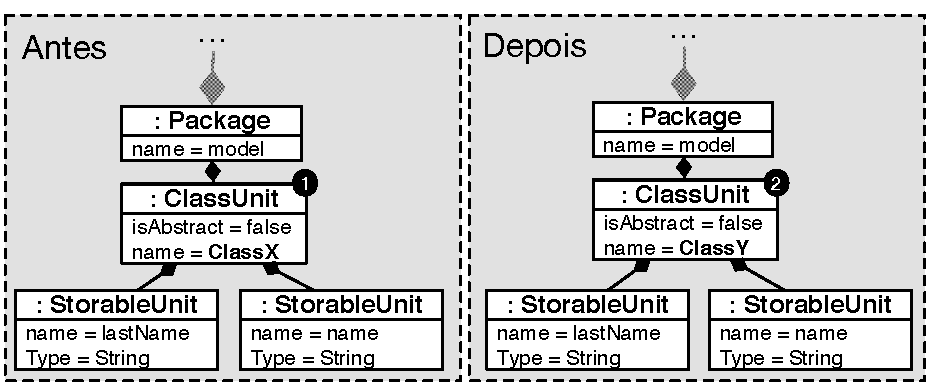
\includegraphics[scale=0.6]{images/antes_depois_refatoracao_renameClassUnit}
	\fautor
	\label{fig:antes_e_depois_rename_classUnit}
\end{minipage}\hfill
			\item Algoritmo: 
			    \begin{itemize}
			        \item \{\texttt{ClassUnit}Selecionada\}.renameClassUnit(\{novoNome\});
			        %\item para cada construtor - \texttt{MethodUnit.Kind=Construtor}.renameMethodUnit(\{novoNome\});
			        %\item para cada referência da \{\texttt{ClassUnit}Selecionada\} deve-se mudar o meta-relacionamento \texttt{to} das metaclasses \texttt{Calls}, \texttt{Creates}, etc. 
			    \end{itemize}
		\end{enumerate}
	\item Especificação Formal:
		\begin{enumerate}
			\item Pré-condição: 
			\begin{codigo}[caption={[OCL representando a pré-condição da refatoração \textit{Rename ClassUnit}.] Pré-condição da refatoração \textit{Rename ClassUnit}.},escapeinside={(*@}{@*)}, basicstyle=\footnotesize, label={codigo:pre_renameClassUnit}, language=OCL]{Name}
context ClassUnit::preRenameClassUnit(newName: String)
pre : newName.isValidadName() 
and not ClassUnit.eContainer.codeElement(*@$\rightarrow$@*)exist (c : ClassUnit | c.name = newName) 
and not ClassUnit.codeElement(*@$\rightarrow$@*)exist (m: MethodUnit | m.name = newName and m.kind =  method)
\end{codigo}

%É importante observar que deve-se especificar a \texttt{ClassUnit} que será renomeada, bem como definir o novo nome dessa \texttt{ClassUnit} antes de executar a pré-condição, como apresentado no Código-fonte~\ref{codigo:pre_renameClassUnit}. 
Na linha 1 do Código-fonte~\ref{codigo:pre_renameClassUnit} é declarado o nome da pré-condição, também é declarado que essa restrição, é apenas executada para instâncias da metaclasse \texttt{ClassUnit}. Na linha 2 verifica-se se o parâmetro \texttt{newName} é um nome válido. Posteriormente, na linha 3 é verificado também se existe outra instância de \texttt{ClassUnit} com o mesmo valor do parâmetro \texttt{newName}. Linha 4 é verificado se existe alguma instância de \texttt{MethodUnit} com o mesmo valor do parâmetro \texttt{newName}. Caso a restrição definida na pré-condição seja válida a refatoração \textit{Rename ClassUnit} é executada.
			\item Algoritmo: 
	\begin{codigo}[caption={[ATL representando a refatoração \textit{Rename ClassUnit}.] ATL da refatoração \textit{Rename ClassUnit}.},escapeinside={(*@}{@*)}, basicstyle=\footnotesize, label={codigo:rename_classUnit_refatoracao}, language=ATL]{Name}
module renameClassUnit;
create OUT : MM refining IN : MM;
rule changeClassUnit {
	from
		source : MM!ClassUnit (source.name = (*@\aspas{\{\texttt{ClassUnit}Selecionada\}}@*))
	to 
		target : MM!ClassUnit (
			name (*@$\leftarrow$@*) (*@\aspas{\{newName\}}@*)
		)
}
\end{codigo}
A refatoração \textit{Rename ClassUnit} é caracterizada pela operação atômica \texttt{change}. Dessa forma, a refatoração foi implementada seguindo o \textit{template} apresentado na Seção~\ref{sec:linguagemDeTransformacaoUtilizada} no Código-fonte~\ref{codigo:template_change}. Dessa forma, o \textit{template} e a Tabela~\ref{tab:guia_template_operacao_change} foram utilizadas para realizar a implementação do Código-fonte~\ref{codigo:rename_classUnit_refatoracao}. Observe que tanto \{\texttt{ClassUnit}Selecionada\} quanto \{\textit{newName}\} são parâmetros que devem ser especificados pelo engenheiro. Assim, foi criado um \textit{plug-in} para auxiliar o engenheiro durante a especificação e execução das refatorações. Maiores informações sobre esse \textit{plug-in} estão no Capítulo~\ref{chapter:ferramenta_kdm_re}.     
			\item Pós-condição:
			 \begin{codigo}[caption={[OCL representando a pós-condição da refatoração \textit{Rename ClassUnit}.] Pós-condição da refatoração \textit{Rename ClassUnit}.},escapeinside={(*@}{@*)}, basicstyle=\footnotesize, label={codigo:pos_condicao_rename_classUnit}, language=OCL]{Name}
 context ClassUnit::RenameClassUnit(newName: String)
 post : name = newName and ClassUnit.eContainer.codeElement(*@$\rightarrow$@*)exist (m : MethodUnit | implies m.name = newName)
\end{codigo}
Na linha 1 do Código-fonte~\ref{codigo:pos_condicao_rename_classUnit} é declarado o nome da pós-condição, também é declarado que essa restrição, é apenas executada para o contexto de instâncias da metaclasse \texttt{ClassUnit}. Na linha 2 o parâmetro \texttt{newName} é comparado com o nome da \texttt{ClassUnit} refatorada, além disso, na linha 2 também é verificado se o construtor também foi alterado o seu nome corretamente. Se ambas as condições foram válidas, a refatoração foi realizada com sucesso.
		\end{enumerate}
\end{enumerate}
		
%--------------------------
\subsection{Refatoração \textit{Push Down StorableUnit}}
Nesta seção a refatoração \textit{Push Down StorableUnit} é apresentada. Essa refatoração é utilizada para remover a generalização de atributos, ou seja, um atributo é apenas utilizado em algumas sub-classes não em todas, assim, não é interessante manter a generalização do atributo na super-classe, uma vez que cada sub-classe pode definir um comportamento para o atributo~\cite{Fowler1999}.

\begin{enumerate}
	\item Especificação Informal:
		\begin{enumerate}
			\item Nome: \textit{Push Down StorableUnit};
			\item Definição:
			    \begin{itemize}
			        \item \texttt{StorableUnit}Selecionado - um atributo que será movido para sub-classes;
			        \item \texttt{ClassUnit} - uma classe na qual o \{\texttt{StorableUnit}Selecionado\} é definido;
			        \item sub-\texttt{ClassUnit}Selecionadas - sub-classes de \{\texttt{ClassUnit}\}.
			    \end{itemize}
			\item Objetivo: Mover um \{\texttt{StorableUnit}Selecionado\} para as \{sub-\texttt{ClassUnit}Selecionadas\}.
			\item Descrição (opcional): \{\texttt{StorableUnit}Selecionado\} é utilizada em apenas algumas sub-classes.
			\item Pré-condição:
			    \begin{itemize}
			        \item \{\texttt{StorableUnit}Selecionado\} não é utilizado em \texttt{ClassUnit};
			        \item as sub-\texttt{ClassUnit}Selecionadas não contêm as mesmas características do \{\texttt{StorableUnit} Selecionado\}, ou seja, os nomes e tipos são diferentes.
			    \end{itemize}
			\item Pós-condição:
			    \begin{itemize}
			        \item \{\texttt{StorableUnit}Selecionado\} não é definido em \texttt{ClassUnit};
			        \item todos os \textit{siblings} de \{\texttt{StorableUnit}Selecionado\} estão definidos nas sub-\texttt{ClassUnit}Selecionadas.
			    \end{itemize}
			\item Mecanismo: Na Figura~\ref{fig:antes_e_depois_pushDown_StorableUnit} duas instâncias simplificada do KDM são ilustradas, a parte superior ilustra a instância antes da realização da refatoração \textit{Push Down StorableUnit} e a parte inferior representa o resultado da refatoração. Como observado, o primeiro passo da refatoração \textit{Push Down StorableUnit} é selecionar um específico \texttt{StorableUnit}, Figura~\ref{fig:antes_e_depois_pushDown_StorableUnit} \ding{202}. Em seguida, deve-se selecionar as sub-classes que realmente utilizam esse \texttt{StorableUnit} para move-lo, com ilustrado na Figura~\ref{fig:antes_e_depois_pushDown_StorableUnit} \ding{203}. Posteriormente o \{\texttt{StorableUnit}Selecionado\} é movido para as sub-\texttt{ClassUnit}Selecionadas, como ilustrado na parte inferior da Figura~\ref{fig:antes_e_depois_pushDown_StorableUnit} \ding{205}. Note que a instância da \texttt{ClassUnit} que havia o \{\texttt{StorableUnit}Selecionado\} não possui mais sua instância, como apresentado na Figura~\ref{fig:antes_e_depois_pushDown_StorableUnit} \ding{204}.
			
			
\begin{minipage}{.90\textwidth}
	\vspace*{\fill}
  \centering
	% Requires \usepackage{graphicx}
	\captionof{figure}{Instância simplificada do KDM antes e depois da refatoração \textit{Push Down StorableUnit}}
	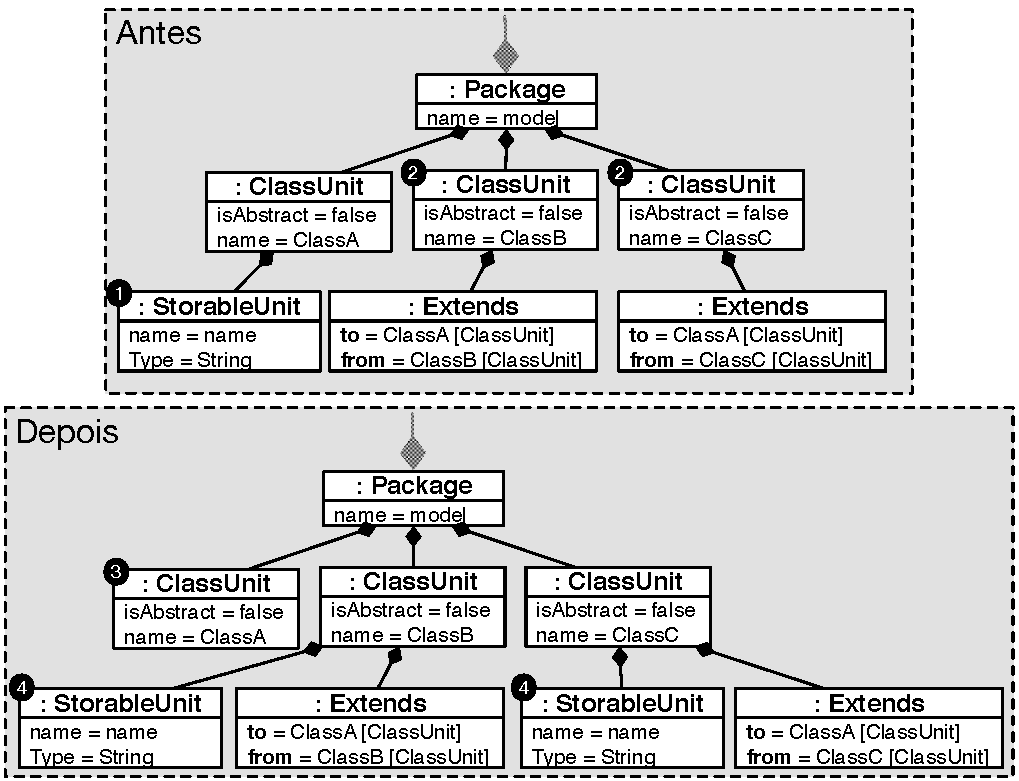
\includegraphics[scale=0.6]{images/pushDownStorableUnitAntesDepois2}
	\fautor
	\label{fig:antes_e_depois_pushDown_StorableUnit}
\end{minipage}\hfill
			\item Algoritmo: 
			    \begin{itemize}
			        \item para cada sub-\texttt{ClassUnit}Selecionadas que realmente usa o \{\texttt{StorableUnit}Selecionado\} - sub-\texttt{ClassUnit}Selecionadas.add(\{\texttt{StorableUnit}Selecionado\})
			        \item \{\texttt{ClassUnit}\}.delete(\{\texttt{StorableUnit}Selecionado\}). 
			    \end{itemize} 
	    \end{enumerate}
		\item Especificação Formal:
		\begin{enumerate}
			\item Pré-condição: 
			\begin{codigo}[caption={[OCL representando a pré-condição da refatoração \textit{Push Down StorableUnit}.] Pré-condição da refatoração \textit{Push Down StorableUnit}.},escapeinside={(*@}{@*)}, basicstyle=\footnotesize, label={codigo:pre_push_down_storableUnit}, language=OCL]{Name}
context StorableUnit::PushDownStorableUnit(subClasses:(ClassUnit))
pre : self.refImmediateComposite().codeElement(*@$\rightarrow$@*)forAll (m: MethodUnit |  not (m.codeRelation(*@$\rightarrow$@*)exists(r: Reads | r.to = self)) 
and not (m.codeRelation(*@$\rightarrow$@*)exists (w:Writes | w.to = self)) 
and not (m.codeRelation(*@$\rightarrow$@*)exists (a: Addresses | a.to = self) 
and subClasses(*@$\rightarrow$@*)forAll (c: ClassUnit | not c.codeElement(*@$\rightarrow$@*)exists(s: StorableUnit | s.name = self.name)))
\end{codigo}



%É importante observar que deve-se especificar a \texttt{ClassUnit} que será renomeada, bem como definir o novo nome dessa \texttt{ClassUnit} antes de executar a pré-condição, como apresentado no Código-fonte~\ref{codigo:pre_renameClassUnit}. 
Na linha 1 do Código-fonte~\ref{codigo:pre_push_down_storableUnit} é declarado a assinatura da pré-condição da refatoração \textit{Push Down StorableUnit}. Note que apenas é utilizado como parâmetro as sub-classes selecionadas para mover o \{\texttt{StorableUnit}Selecionado\}. Na linha 2 a instância da \texttt{ClassUnit} que contém o \{\texttt{StorableUnit}Selecionado\} é obtida por meio da função \texttt{refImmediateComposite()}. Posteriormente, todas as instâncias de \texttt{MethodUnit} são obtidas para realizar uma iteração. Ainda na linha 2, essa iteração verifica se o \{\texttt{StorableUnit}Selecionado\} é lido em alguma instância de \texttt{MethodUnit}. Similarmente, na linha 3 e 4 todos os \texttt{MethodUnits} são verificados para identificar se o \{\texttt{StorableUnit}Selecionado\} é escrito e utilizado. Na linha 5 todas as \{sub-\texttt{ClassUnit}Selecionadas\} são verificadas para identificar se existe uma instância similar ao \{\texttt{StorableUnit}Selecionado\} antes de realizar a refatoração. Caso a pré-condição definida seja válida a refatoração \textit{Push Down StorableUnit} é executada.
			\item Algoritmo: 
	\begin{codigo}[caption={[ATL representando a refatoração \textit{Push Down StorableUnit}.] ATL da refatoração \textit{Push Down StorableUnit}.},escapeinside={(*@}{@*)}, basicstyle=\footnotesize, label={codigo:push_Down_StorableUnit_ATL}, language=ATL]{Name}
module pushDownStorableUnit;
create OUT : MM refining IN : MM;
rule createStorableUnit {
	from
		source : MM!ClassUnit (source.name = (*@\aspas{\{sub-\texttt{ClassUnit}Selecionada\}}@*)
	to 
		target : MM!ClassUnit (
			codeElement(*@$\leftarrow$@*)source.codeElement(*@$\rightarrow$@*)including(newElement)
		),
		newElement: MM!StorableUnit (
			name(*@$\leftarrow$@*)(*@\{\texttt{StorableUnit}Selecionado.name\}@*),
			type(*@$\leftarrow$@*)(*@\{\texttt{StorableUnit}Selecionado.type\}@*)
		)
}
rule deleteStorableUnit {
	from
		source : MM!StorableUnit (source.name = (*@\{\texttt{StorableUnit}Selecionado.name\}@*) and source.refImmediateComposite().name = (*@\{\texttt{ClassUnit}.name\}@*) )
	to
		drop
}
\end{codigo}
O Código-fonte~\ref{codigo:push_Down_StorableUnit_ATL} apresenta a refatoração \texttt{Push Down StorableUnit}. Como apresentado na Tabela~\ref{tab:refatoringsCatalogo} essa refatoração pode ser implementada pela combinação de duas operações atômicas: (\textit{i}) \texttt{add} e \texttt{delete}. Dessa forma, os \textit{templates} apresentados nos Códigos-fontes~\ref{codigo:template_addKDMElement} e \ref{codigo:template_delete} foram utilizados como guia para implementar essa refatoração.
%Na linha 1 do Código-fonte~\ref{codigo:push_Down_StorableUnit_ATL} o nome da refatoração é definido. Em seguida, na linha 2 é apresentado o cabeçalho da refatoração, novamente a palavra-chave \textit{refining} é especificada para informar que a transformação/refatoração é do tipo endógenas (ver Capítulo~\ref{chapter:fundamentacao_teorica} Seção~\ref{sec:transformacoes_de_modelos}). Posteriormente, nas linhas 3 até 13 a primeira regra dessa refatoração é definida. Na linha 5 uma condição de guarda é definida para identificar quais são as \{sub-\texttt{ClassUnit}Selecionadas\}. Em seguida, linhas 7, 8 e 9 informa que uma nova instância de \texttt{StorableUnit} será criado nas \{sub-\texttt{ClassUnit}Selecionadas\}. Nas linhas 10, 11 e 12 os meta-atributos do \{\texttt{StorableUnit}Selecionado\} são copiados. Após mover o \{\texttt{StorableUnit}Selecionado\} para as sub-classes, o próximo passo é remover o \{\texttt{StorableUnit}Selecionado\} da super-classe. Esse passo é representado na regra descrita nas linhas 15 até 20. Na linha 17 o \{\texttt{StorableUnit}Selecionado\} é identificado, depois na linha 19 a palavra-chave \textit{drop} é utilizada, a qual especifica que uma determinada instância será removida, neste caso o \{\texttt{StorableUnit}Selecionado\}.   
			\item Pós-condição:
			 \begin{codigo}[caption={[OCL representando a pós-condição da refatoração \textit{Push Down StorableUnit}.] Pós-condição da refatoração \textit{Push Down StorableUnit}.},escapeinside={(*@}{@*)}, basicstyle=\footnotesize, label={codigo:pos_condicao_pushDown_StorableUnit}, language=OCL]{Name}
context StorableUnit::PushDownStorableUnit(subClasses:Bag(ClassUnit))
post : self.refImmediateComposite().codeElement(*@$\rightarrow$@*)exists (s: StorableUnit | not (s.name = self.name)) 
and subClasses->forAll (c: ClassUnit | c.codeElement(*@$\rightarrow$@*)exists (s: StorableUnit | s.name = self.name and s.type = self.type))
\end{codigo}
Na linha 1 do Código-fonte~\ref{codigo:pos_condicao_pushDown_StorableUnit} é declarado o nome da pós-condição. Na linha 2 é verificado se o \{\texttt{StorableUnit}Selecionado\} ainda está na super-classe. Posteriormente, na linha 3, para todas as \{sub-\texttt{ClassUnit}Selecionadas\} são verificadas para garantir que o \{\texttt{StorableUnit}Selecionado\} foi adicionado corretamente. Caso afirmativo a refatoração foi realizada com sucesso.
		\end{enumerate}
	\end{enumerate}		
	
	
	
%--------------------------
\subsection{Refatoração \textit{Extract ClassUnit}}
Nesta seção a refatoração \textit{Extract ClassUnit} é apresentada. Essa refatoração é utilizada quando uma determinada classe está fazendo o trabalho que deveria ser realizada por duas classes~\cite{Fowler1999}. 

\begin{enumerate}
	\item Especificação Informal:
		\begin{enumerate}
			\item Nome: \textit{Extract ClassUnit};
			\item Definição:
			    \begin{itemize}
			        \item \texttt{ClassUnit}Selecionada - a classe que contém os atributos e métodos que devem ser movido para a nova classe;
			        \item novoNome - um novo nome para a nova classe a ser criada;
			        \item \texttt{StorableUnit}Selecionados - atributos relevantes selecionados para serem movido para a nova classe;
			        \item \texttt{MethodUnit}Selecionados - métodos relevantes selecionados para serem movidos para a nova classe.
			    \end{itemize}
			\item Objetivo: Criar uma nova \texttt{ClassUnit} e mover os \texttt{StorableUnit}Selecionados e \texttt{MethodUnit}Selecionados para esse nova instância.
			\item Descrição (opcional): \texttt{ClassUnit}Selecionada está realizando o trabalho que deveria ser realizado por duas classes.
			\item Pré-condição:
			    \begin{itemize}
			        \item \{\texttt{ClassUnit}Selecionada\} deve contém atributos e métodos para mover para a nova classe;
			        \item os \{\texttt{StorableUnit}Selecionados\} não são utilizados na \{\texttt{ClassUnit}Selecionada\};
			        \item os \{\texttt{MethodUnit}Selecionados\} não são utilizados na \{\texttt{ClassUnit}Selecionada\};
			        \item o \{novoNome\} da nova instância da \texttt{ClassUnit} deve seguir as convenções válidas para nomes de classes;
			        \item não deve existir outra instância da \texttt{ClassUnit} com o mesmo nome dentro do mesmo \texttt{Package}.
			    \end{itemize}
			\item Pós-condição:
			    \begin{itemize}
			        \item \{\texttt{StorableUnit}Selecionados\} não são definido em \{\texttt{ClassUnit}Selecionada\};
			        \item \{\texttt{MethodUnit}Selecionados\} não são definido em \{\texttt{ClassUnit}Selecionada\};
			        \item todos os \{\texttt{StorableUnit}Selecionados\} e \{\texttt{MethodUnit}Selecionados\} estão definidos na nova instância da \texttt{ClassUnit} criada.
			    \end{itemize}
			\item Mecanismo: O primeiro passo da refatoração \textit{Extract ClassUnit} é selecionar um conjunto de \texttt{StorableUnits} e/ou \texttt{MethodUnits} que serão adicionados para uma nova instância de metaclasse \texttt{ClassUnit}, no exemplo ilustrado na Figura~\ref{fig:antes_e_depois_extract_ClassUnit} \ding{202} duas instâncias de \texttt{StorableUnits} são selecionadas. Posteriormente, uma nova instância da metaclasse \texttt{ClassUnit} é criada e adicionada ao mesmo \texttt{Package} que a instância da metaclasse \texttt{ClassUnit} e que contém os \{\texttt{StorableUnit}Selecionados\}, como ilustrado na Figura~\ref{fig:antes_e_depois_extract_ClassUnit} \ding{204}. Em seguida, todos os \{\texttt{StorableUnit}Selecionados\} são adicionados nessa nova instância, como representado na Figura~\ref{fig:antes_e_depois_extract_ClassUnit} \ding{203}. %Em seguida, deve-se deletar os \{\texttt{StorableUnit}Selecionados\}.
\begin{minipage}{.90\textwidth}
	\vspace*{\fill}
  \centering
	% Requires \usepackage{graphicx}
	\captionof{figure}{Instância simplificada do KDM antes e depois da refatoração \textit{Extract ClassUnit}}
	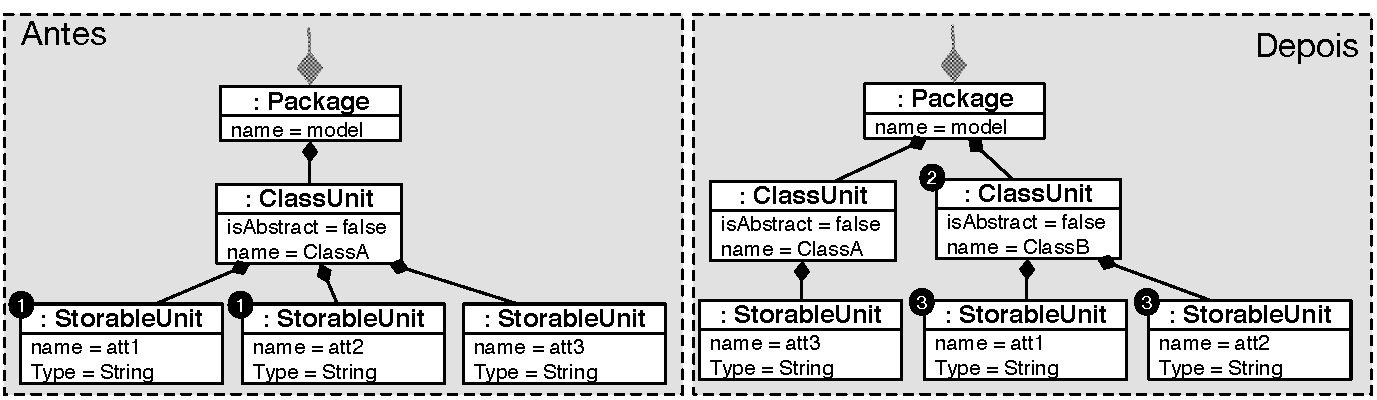
\includegraphics[scale=0.6]{images/extractClassUnitAntesEDepois2}
	\fautor
	\label{fig:antes_e_depois_extract_ClassUnit}
\end{minipage}\hfill
			\item Algoritmo: 
			    \begin{itemize}
			        \item addNewClassUnit(\{novoNome\});
			        \item adiciona essa nova instância dentro de um \texttt{Package};
			        \item para cada \{\texttt{StorableUnit}Selecionado\} - move(\{newClassUnit\}, \{\texttt{StorableUnit}Selecionado\})
			        \item para cada \{\texttt{MethodUnit}Selecionado\} - move(\{newClassUnit\}, \{\texttt{MethodUnit}Selecionado\});
			        \item createNewHasType(\{newClassUnit\}, \{\texttt{ClassUnit}Selecionada\}).
			    \end{itemize} 
	    \end{enumerate}
		\item Especificação Formal:
		\begin{enumerate}
			\item Pré-condição: 
			\begin{codigo}[caption={[OCL representando a pré-condição da refatoração \textit{Extract ClassUnit}.] Pré-condição da refatoração \textit{Extract ClassUnit}.},escapeinside={(*@}{@*)}, basicstyle=\footnotesize, label={codigo:pre_extract_ClassUnit}, language=OCL]{Name}
context ClassUnit::ExtractClassUnit(newName: String, storableUnitSelected:(StorableUnit), methodUnitSelected: (MethodUnit))
pre : newName.isValidName() and not self.refImmediateComposite().codeElement(*@$\rightarrow$@*)exist (c: ClassUnit | c.name = newName) 
and not storableUnitSelected(*@$\rightarrow$@*)forAll (s: StorableUnit | self.codeElement(*@$\rightarrow$@*)forAll (m: MethodUnit | not (m.codeRelation(*@$\rightarrow$@*)exists(re: Reads | re.to = s)) and not (m.codeRelation(*@$\rightarrow$@*)exists (wr:Writes | wr.to = s)) and not (m.codeRelation(*@$\rightarrow$@*)exists (add: Addresses | add.to = s)) 
and not methodUnitSelected(*@$\rightarrow$@*)forAll (m: MethodUnit | self.codeElement(*@$\rightarrow$@*)forAll (m: MethodUnit | not (m.codeRelation(*@$\rightarrow$@*)exists (call: Calls| call.to = m)))))
\end{codigo}
%É importante observar que deve-se especificar a \texttt{ClassUnit} que será renomeada, bem como definir o novo nome dessa \texttt{ClassUnit} antes de executar a pré-condição, como apresentado no Código-fonte~\ref{codigo:pre_renameClassUnit}. 
Na linha 1 do Código-fonte~\ref{codigo:pre_extract_ClassUnit} é declarado a assinatura da pré-condição da refatoração \textit{Extract ClassUnit}, note que essa pré-condição possui três parâmetros: o nome da nova instância da metaclasse \texttt{ClassUnit}, um conjunto de \{\texttt{StorableUnit}Selecionado\} e um conjunto de \{\texttt{MethodUnit}Selecionado\}. Na linha 2 é verificado se o parâmetro \{newName\} é válido para ser utilizado como nome de classe. Ainda na linha 2 a instância de da metaclasse \texttt{Package} é obtida por meio da função \texttt{refImmediateComposite()} para verificar dentro do escopo deste pacote se não existe nenhuma classe com o mesmo nome. Na linha 3 para cada \{\texttt{StorableUnit}Selecionado\} é verificado se são utilizados dentro de uma instância de \texttt{MethodUnit}, ou seja, verifica-se se o \{\texttt{StorableUnit}Selecionado\} é escrito e utilizado nos métodos. Similarmente, na linha 4 é verificado para cada \{\texttt{MethodUnit}Selecionado\} se o mesmo é chamado em algum lugar. Caso a pré-condição definida seja válida a refatoração \textit{Extract ClassUnit} é executada.
			\item Algoritmo: 
	\begin{codigo}[caption={[ATL representando a refatoração \textit{Extract ClassUnit}.] ATL da refatoração \textit{Extract ClassUnit}.},escapeinside={(*@}{@*)}, basicstyle=\footnotesize, label={codigo:extract_classUnit_ATL}, language=ATL]{Name}
module createAnClassThenMoveAnAttribute;
create OUT : MM refining IN : MM;
rule extractClassUnit {
	from
		source : MM!Package (source.name = (*@\aspas{\{\texttt{ClassUnit}Selecionada.refImmediateComposite()\}}@*))
	to 
		target: MM!Package (
			codeElement(*@$\leftarrow$@*)source.codeElement(*@$\rightarrow$@*)including(newClassUnit)
		),
		newClassUnit: MM!ClassUnit (
			name(*@$\leftarrow$@*)(*@\aspas{\{newName\}}@*),
			codeElement(*@$\leftarrow$@*)thisModule.getMethodUnits(thisModule.getClassUnit((*@\aspas{\{\texttt{ClassUnit}Selecionada\}}@*)), (*@\aspas{\{\texttt{MethodUnit}Selecionados\}}@*)),
			codeElement(*@$\leftarrow$@*)thisModule.getStorableUnits(thisModule.getClassUnit((*@\aspas{\{\texttt{ClassUnit}Selecionada\}}@*)), (*@\aspas{\{\texttt{StorableUnit}Selecionados\}}@*)))
rule createLinkExtractClassUnit {
	from
		source : MM!ClassUnit (source.name = (*@\aspas{\{\texttt{ClassUnit}Selecionada\}}@*))
	to 
		target: MM!ClassUnit (
			codeRelation(*@$\leftarrow$@*)source.codeRelation(*@$\rightarrow$@*)including(hasType)
		),
		hasType: MM!HasType (
			to(*@$\leftarrow$@*)(*@\aspas{\{\texttt{ClassUnit}Selecionada\}}@*),
			from(*@$\leftarrow$@*)(*@\aspas{\{new\texttt{ClassUnit}\}}@*)
		)
}}
helper def : getClassUnit (className : String) : MM!ClassUnit = MM!ClassUnit.allInstances()->any(e | e.name = className);
helper def : getStorableUnit (classUnitToGetTheStorableUnit: MM!ClassUnit, nameOfAtt: String) : MM!StorableUnit = classUnitToGetTheStorableUnit.codeElement(*@$\rightarrow$@*)any(e | e.name = nameOfAtt);		
helper def : getMethodUnits (classUnitToGet: MM!ClassUnit, nameMethod: String) : MM!MethodUnit = classUnitToGet.codeElement(*@$\rightarrow$@*)any(e | e.name.equalsIgnoreCase(nameMethod));
\end{codigo}
Na linha 1 do Código-fonte~\ref{codigo:extract_classUnit_ATL} o nome da refatoração é definido. Em seguida, na linha 2 é apresentado o cabeçalho da refatoração. Nas linhas 3 até 13 a primeira regra dessa refatoração é definida. Na linha 5 uma condição de guarda é definida para identificar a instância da metaclasse \texttt{Package} que a nova instância da metaclasse \texttt{ClassUnit} será adicionada. Em seguida, as linhas 7, 8 e 9 representam que uma nova instância de \texttt{StorableUnit} será criado dentro da instância do \texttt{Package} identificado. Nas linhas 10 e 11 uma nova instância da metaclasse \texttt{ClassUnit} é efetivamente criada. Posteriormente, nas linhas 12 e 13 os \{\texttt{StorableUnit}Selecionados\} e os \{\texttt{MethodUnit}Selecionados\} são movidos para a \texttt{ClassUnit} recém instanciada. Após mover os \{\texttt{StorableUnit}Selecionados\} e os \{\texttt{MethodUnits}Selecionados\} para a \texttt{ClassUnit} o próximo passo é criar uma associação entre as duas instâncias de \texttt{ClassUnit}. Esse passo é representado na regra descrita nas linhas 14 até 25. Na linha 17 a {\texttt{ClassUnit}Selecionada\} é identificada, depois as linhas 18, 19 e 20 sinalizam que uma instância da metaclasse \texttt{HasType} será criada. Finalmente, nas linhas 21 até 23 a instância da metaclasse \texttt{HasType} é criada. Mas especificadamente, nas linhas 22 e 23 seus relacionamentos \texttt{to} e \texttt{from} são definidos, os quais representam a associação entre a classe que continha os \{\texttt{StorableUnit}Selecionados\} e os \{\texttt{MethodUnits}Selecionados\} e a nova instância da metaclasse \texttt{ClassUnit}, respectivamente. Linhas 26, 27 e 28 os \textit{helpers} que são utilizadas nessa refatoração são definidos.   
			\item Pós-condição:
			 \begin{codigo}[caption={[OCL representando a pós-condição da refatoração \textit{Extract ClassUnit}.] Pós-condição da refatoração \textit{Extract ClassUnit}.},escapeinside={(*@}{@*)}, basicstyle=\footnotesize, label={codigo:pos_condicao_extract_ClassUnit}, language=OCL]{Name}
context ClassUnit::ExtractClassUnit(storableUnitSelected: (StorableUnit), methodUnitSelected: (MethodUnit), newClass: ClassUnit)
post : self.codeElement(*@$\rightarrow$@*)exists (s: StorableUnit | not (storableUnitSelected(*@$\rightarrow$@*)forAll (sUS: StorableUnit | sUS.name = s.name))) and self.codeElement(*@$\rightarrow$@*)exists (m: MethodUnit | not (methodUnitSelected(*@$\rightarrow$@*)forAll (mUS: MethodUnit | mUS.name = m.name))) 
and newClass.codeElement(*@$\rightarrow$@*)exist (s: StorableUnit | (storableUnitSelected(*@$\rightarrow$@*)forAll (sUS: StorableUnit | sUS.name = s.name))) and newClass.codeElement(*@$\rightarrow$@*)exists (m: MethodUnit | not (methodUnitSelected(*@$\rightarrow$@*)forAll (mUS: MethodUnit | mUS.name = m.name)))        \end{codigo}
Na linha 1 do Código-fonte~\ref{codigo:pos_condicao_extract_ClassUnit} é declarado o nome da pós-condição. Na linha 2 é verificado se todos os \{\texttt{StorableUnit}Selecionados\} e \{\texttt{MethodUnits}Selecionados\} não estão definidos na \{\texttt{ClassUnit}Selecionada\}. Posteriormente, na linha 3, é verificado se todos os \{\texttt{StorableUnit}Selecionados\} e \{\texttt{MethodUnits}Selecionados\} foram efetivamentes movidos para a nova instância da metaclasse \texttt{ClassUnit}. Caso afirmativo a refatoração foi realizada com sucesso.
		\end{enumerate}
\end{enumerate}
	
	
\section{Considerações Finais}\label{sec:consideracoes_finais_capitulo_reforacao}

Neste capítulo foram apresentadas cinco diretrizes para auxiliar o engenheiro de modernização a criar refatorações para o metamodelo KDM. Com o intuito de exemplificar essas cinco diretrizes foram escolhidas algumas refatorações propostas por~\citeonline{Fowler1999} para serem criadas para o metamodelo KDM. Embora ~\citeonline{Fowler1999} tenha definido um catálogo de refatoração para ser utilizado em código-fonte, mais de 60\% das refatorações (44 de 72) são ilustradas e explicadas utilizando modelos, mais especificadamente diagramas de classes da UML. Esta observação fez com que tais refatorações fossem criadas para o metamodelo KDM. 

Antes de criar qualquer refatoração para o metamodelo KDM, a primeira diretrizes diz que é  necessário identificar as metaclasses do KDM que têm características similares aos conceitos do POO, bem como instruções comumente utilizadas em todas as linguagens de programação, tais como, ramificações, iterações, etc. Dessa forma, esse capítulo também apresentou um mapeamento entre os conceitos do POO e o metamodelo KDM. Acredita-se que engenheiros de modernização pouco familiarizado com o metamodelo KDM podem gastar menos tempo durante a criação de novas refatorações com a utilização deste mapeamento, assim, qualquer exemplo de refatoração pode ser facilmente adaptada para o metamodelo KDM seguindo esse mapeamento, bem como as diretrizes aqui apresentadas.

Após identificar todos os elementos estruturais e identificar o mapeamento entre POO e o metamodelo KDM, o próximo passo é escolher qual refatoração criar. No contexto desta Tese todas as refatorações podem ser agrupadas em nível de granularidade. As granularidades podem ser definidas em dois níveis de operações: (\textit{i}) operação atômica e (\textit{ii}) operações compostas. As granularidades definidas como operações atômicas podem ser especificas por meio de operações primitivas (\texttt{addd}, \texttt{delete} e \texttt{change}). As refatorações de granularidade compostas são uma combinação de operações atômicas (ver Tabela~\ref{tab:refatoringsCatalogo}). Em seguida na próxima diretriz o engenheiro de modernização deve implementar a refatoração por meio da linguagem de transformação ATL. Então o engenheiro de modernização deve implementar as restrições (pré- e pós-condições) da refatoração.

Após criar uma determinada refatoração, bem como suas pré- e pós-condições para o metamodelo KDM, o engenheiro de modernização deve especificar e documentar a refatoração. As refatoração criadas para o metamodelo KDM consistem de duas principais especificações - uma especificação informal e uma especificação formal. Na especificação informal a ideologia básica é permitir que o engenheiro de modernização expresse o propósito da refatoração por meio de linguagem natural. A segunda especificação é responsável por representar as pré- e pós-condições, bem como a transformação/refatoração propriamente dita em linguagens executáveis - OCL e ATL foram utilizadas, respectivamente. Ambas especificações são úteis para o engenheiro de modernização -a especificação informal é utilizada para facilitar a compreensão e o propósito da refatoração,enquanto que a especificação formal facilita a implementação da refatoração. Além disso, a especificação formal é de extrema importância para facilitar a automação das refatorações. %É importante destacar que neste capítulo apenas as refatorações \textit{Rename ClassUnit}, \textit{Pull Up StorableUnit}, \textit{Push Down StorableUnit} e \textit{Extract ClassUnit} são apresentadas e detalhadas.

Seguindo as diretrizes apresentada neste capítulo o engenheiro de modernização pode criar refatorações para o metamodelo KDM. No entanto, as especificações formais e informais resultantes não são suficientes para promover o reúso de refatorações no contexto do metamodelo KDM. Dessa forma, no Capítulo~\ref{chapter:Toward_a_Refactoring_Metamodel_for_KDM} é apresentado um metamodelo para auxiliar o engenheiro de modernização a promover o reúso de refatorações no contexto do metamodelo KDM. Com a utilização desse metamodelo, informações (metadados) sobre refatorações podem ser reutilizadas de forma independente de linguagem e plataforma. No Capítulo~\ref{chapter:Abordagem_de_sincronizacao} uma abordagem para manter instâncias do metamodelo KDM sincronizada e consiste após a aplicação de refatoração é apresentada. No Capítulo~\ref{chapter:ferramenta_kdm_re} é apresentado uma ferramenta que foi desenvolvida dentro do ambiente Eclipse para apoiar o uso do catálogo de refatoração adaptado para o metamodelo KDM, dessa forma, essa ferramenta permite que modernizadores apliquem refatorações diretamente no metamodelo KDM. 
